\documentclass[../../main.tex]{subfiles}

\graphicspath{{../../image/}{../../figure/}}

\begin{document}

\section{多元 Gauss 分布}\label{section:ch03-多元Gauss分布}

Gauss 分布又称正态分布，已广泛用于建模连续变量的分布。我们已经看到对于单个变量 $x$（参见\cref{section:ch02-Gauss分布}），Gauss 分布可以写为如下形式：
\begin{align}
\mathcal{N}(x\mid\mu,\sigma^{2})=\frac{1}{(2\pi\sigma^{2})^{1/2}}\exp\left\{-\frac{1}{2\sigma^{2}}(x-\mu)^{2}\right\},
\label{align:ch03-一元Gauss}
\end{align}
其中 $\mu$ 是均值，$\sigma^{2}$ 是方差。对于一个 $D$ 维向量 $\boldsymbol{x}$，多元 Gauss 分布有如下形式：
\begin{align}
\mathcal{N}(\boldsymbol{x}\mid\boldsymbol{\mu},\boldsymbol{\Sigma})=\frac{1}{(2\pi)^{D/2}\lvert\boldsymbol{\Sigma}\rvert^{1/2}}\exp\left\{-\frac{1}{2}(\boldsymbol{x}-\boldsymbol{\mu})^{\mathsf{T}}\boldsymbol{\Sigma}^{-1}(\boldsymbol{x}-\boldsymbol{\mu})\right\},
\label{align:ch03-多元Gauss}
\end{align}
其中 $\boldsymbol{\mu}$ 是 $D$ 维均值向量，$\boldsymbol{\Sigma}$ 是 $D\times D$ 的协方差矩阵，$\lvert\boldsymbol{\Sigma}\rvert$ 表示 $\boldsymbol{\Sigma}$ 的行列式。

\begin{definition}[多元 Gauss 分布]\label{definition:ch03-多元Gauss分布}
设 $\boldsymbol{\mu}\in\mathbb{R}^{D}$，$\boldsymbol{\Sigma}$ 为 $D\times D$ 的对称正定矩阵。则称由\eqref{align:ch03-多元Gauss}定义的密度为均值 $\boldsymbol{\mu}$、协方差 $\boldsymbol{\Sigma}$ 的多元 Gauss 分布，记作 $\mathcal{N}(\boldsymbol{x}\mid\boldsymbol{\mu},\boldsymbol{\Sigma})$。
\end{definition}

% SUPPLEMENT: parent=definition:ch03-多元Gauss分布; kind=motivation; location=紧随其后的 remark（重构新增）
\begin{remark}（重构新增）
多元 Gauss 分布是把一元 Gauss 分布\eqref{align:ch03-一元Gauss}中的“标量平方”换成“二次型”得到的：$(x-\mu)^{2}/\sigma^{2}$ 变为 $(\boldsymbol{x}-\boldsymbol{\mu})^{\mathsf{T}}\boldsymbol{\Sigma}^{-1}(\boldsymbol{x}-\boldsymbol{\mu})$，而 $\sigma^{2}$ 则被 $\boldsymbol{\Sigma}$ 取代。这一替换并非任意：它使得等密度面成为椭球（\cref{subsection:ch03-Gauss几何}），并使 $\boldsymbol{\Sigma}$ 恰为 $\boldsymbol{x}$ 的协方差矩阵（\cref{subsection:ch03-矩}）。

定义要求 $\boldsymbol{\Sigma}$ 对称正定，有两点理由。其一是归一化：归一化系数 $(2\pi)^{-D/2}\lvert\boldsymbol{\Sigma}\rvert^{-1/2}$ 要求 $\lvert\boldsymbol{\Sigma}\rvert>0$；若 $\boldsymbol{\Sigma}$ 奇异，则逆矩阵不存在，密度无法定义。其二是唯一性：若 $\boldsymbol{\Sigma}$ 不对称，则只有它的对称部分 $(\boldsymbol{\Sigma}+\boldsymbol{\Sigma}^{\mathsf{T}})/2$ 会出现在二次型中，非对称部分对密度毫无影响，因此把它纳入参数只会造成不可辨识（\cref{exercise:ch03-11}给出了严格论证）。
\end{remark}

在很多不同的场景中都可以看到 Gauss 分布，因此可以从各种不同的角度来理解它的作用（参见\cref{section:ch02-信息论}）。例如，我们已经看到，对于单个实数变量，能够使它的熵最大化的分布就是 Gauss 分布。这一性质对于多元 Gauss 分布同样适用（见\cref{exercise:ch03-08}）。

当我们考虑多个随机变量之和的时候，同样会用到 Gauss 分布。中心极限定理（central limit theorem）告诉我们，在某些温和的条件下，一组随机变量的和（它本身也是一个随机变量）的分布会随着其中随机变量数量的增加而越来越接近于 Gauss 分布（Walker, 1969）。我们可以这样解释这一现象：有 $N$ 个随机变量 $x_1,\cdots,x_N$，每个随机变量都在 $[0,1]$ 区间上服从均匀分布，考虑均值 $(x_1+\cdots+x_N)/N$ 的分布。对于较大的 $N$，如\cref{figure:ch03-中心极限直方图}所示，这一分布趋向于 Gauss 分布。现实中，随着 $N$ 的增大，分布会很快地收敛到 Gauss 分布。这一结果揭示了\cref{align:ch03-二项分布}中关于变量 $m$ 的二项分布，其中 $m$ 是二元随机变量 $x$ 的 $N$ 个观测样本的和，分布会在 $N\to\infty$ 时趋向于 Gauss 分布（见\cref{figure:ch03-二项分布直方图}中 $N=10$ 的情形）。

\begin{figure}[htbp]
  \centering
  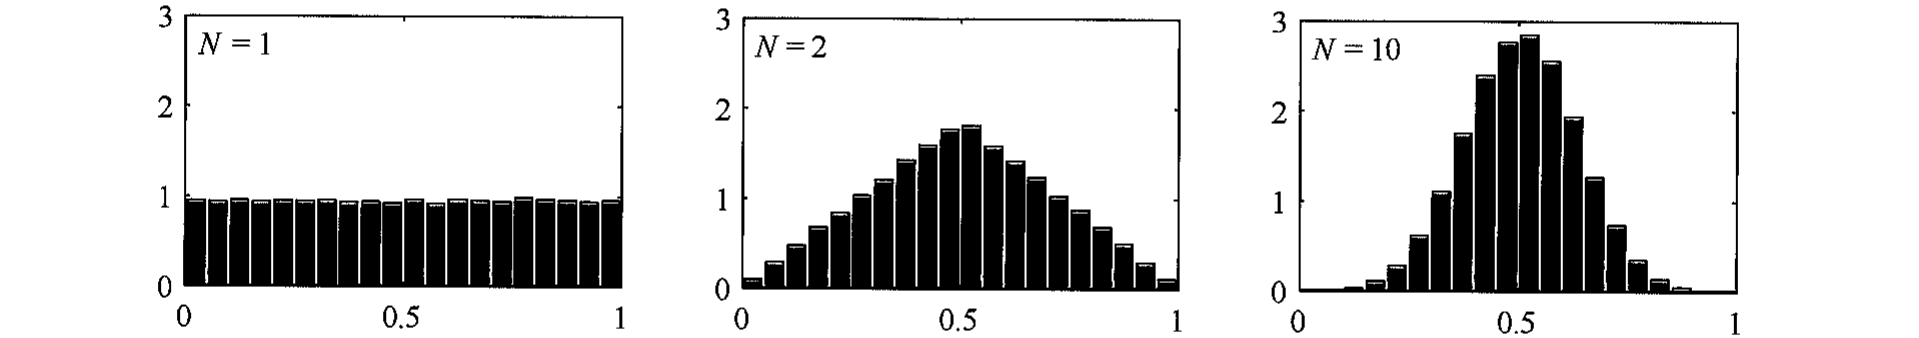
\includegraphics[width=0.92\textwidth]{ch03-fig3-2-clt-hist.png}
  \caption{$N$ 个均匀分布的数字的均值直方图。我们可以看到，随着 $N$ 的增加，分布趋向于 Gauss 分布。}
  \label{figure:ch03-中心极限直方图}
\end{figure}

Gauss 分布有很多重要的分析性质，我们将会考虑其中一些性质的具体细节。因此，本节比前几节更具技术性，读者需要熟悉多种矩阵相关的等式（参见\cref{section:appA-矩阵恒等式}）。

\subsection{Gauss 几何}\label{subsection:ch03-Gauss几何}

下面我们考虑 Gauss 分布的几何形式。Gauss 分布对 $\boldsymbol{x}$ 的函数依赖是通过二次形式来呈现的：
\begin{align}
\Delta^{2}=(\boldsymbol{x}-\boldsymbol{\mu})^{\mathsf{T}}\boldsymbol{\Sigma}^{-1}(\boldsymbol{x}-\boldsymbol{\mu}).
\label{align:ch03-马氏距离}
\end{align}

\begin{definition}[Mahalanobis 距离]\label{definition:ch03-马氏距离}
设 $\boldsymbol{\Sigma}$ 为对称正定矩阵，$\boldsymbol{\mu}\in\mathbb{R}^{D}$。对 $\boldsymbol{x}\in\mathbb{R}^{D}$，称由\eqref{align:ch03-马氏距离}定义的 $\Delta^{2}$ 的算术平方根 $\Delta$ 为 $\boldsymbol{\mu}$ 到 $\boldsymbol{x}$ 的 Mahalanobis 距离。
\end{definition}

% SUPPLEMENT: parent=definition:ch03-马氏距离; kind=motivation; location=紧随其后的 remark（重构新增）
\begin{remark}（重构新增）
引入 Mahalanobis 距离是为了把“距离”从各向同性的欧氏度量推广到由数据分布决定度量的情形：在概率密度高的方向上，同样的坐标差对应更小的 $\Delta$，因此“偏离多少个标准差”才是它度量的东西。当 $\boldsymbol{\Sigma}$ 为单位矩阵时 $\Delta^{2}=\lVert\boldsymbol{x}-\boldsymbol{\mu}\rVert^{2}$，它退化为欧氏距离；当 $\boldsymbol{\Sigma}$ 为对角矩阵时，$\Delta^{2}=\sum_{i}(x_i-\mu_i)^{2}/\sigma_i^{2}$，即各坐标按标准差的加权平方和。

Gauss 分布在 $\boldsymbol{x}$ 空间中的等值面就是 $\Delta$ 为常数的曲面，因为该二次型为常数。定义中的正定性保证了 $\boldsymbol{\Sigma}^{-1}$ 存在且 $\Delta^{2}\geqslant0$，从而 $\Delta$ 是良定义的实数量。
\end{remark}

首先，注意可以不失一般性地假设矩阵 $\boldsymbol{\Sigma}$ 为对称矩阵，因为任何非对称的成分都会从指数中消失（见\cref{exercise:ch03-11}）。考虑协方差矩阵的特征方程：
\begin{align}
\boldsymbol{\Sigma}\boldsymbol{u}_{i}=\lambda_{i}\boldsymbol{u}_{i},
\label{align:ch03-特征方程}
\end{align}
其中 $i=1,\cdots,D$。由于 $\boldsymbol{\Sigma}$ 是实对称矩阵，其特征值是实数，并且其特征向量可以正交化（见\cref{exercise:ch03-12}），故有
\begin{align}
\boldsymbol{u}_{i}^{\mathsf{T}}\boldsymbol{u}_{j}=I_{ij},
\label{align:ch03-特征向量正交}
\end{align}
其中 $I_{ij}$ 是单位矩阵中的元素，满足
\begin{align}
I_{ij}=\begin{cases}1, & \text{当 } i=j \text{ 时},\\ 0, & \text{其他}.\end{cases}
\label{align:ch03-单位矩阵元素}
\end{align}

\begin{proposition}[实对称协方差矩阵的谱性质]\label{proposition:ch03-协方差谱分解}
设 $\boldsymbol{\Sigma}$ 为 $D\times D$ 实对称矩阵。则 $\boldsymbol{\Sigma}$ 的全部特征值 $\lambda_i$ 都是实数，且存在一组标准正交的特征向量 $\{\boldsymbol{u}_i\}$ 使\eqref{align:ch03-特征方程}与\eqref{align:ch03-特征向量正交}同时成立。进一步，$\boldsymbol{\Sigma}$ 可以表示为其特征向量的展开
\begin{align}
\boldsymbol{\Sigma}=\sum_{i=1}^{D}\lambda_{i}\boldsymbol{u}_{i}\boldsymbol{u}_{i}^{\mathsf{T}},
\label{align:ch03-协方差谱分解}
\end{align}
而当 $\boldsymbol{\Sigma}$ 可逆时，其逆矩阵可以表示为
\begin{align}
\boldsymbol{\Sigma}^{-1}=\sum_{i=1}^{D}\frac{1}{\lambda_{i}}\boldsymbol{u}_{i}\boldsymbol{u}_{i}^{\mathsf{T}}.
\label{align:ch03-逆协方差谱分解}
\end{align}
\end{proposition}
\begin{proof}
（重构新增）特征值为实数、特征向量可正交化这两点就是\cref{exercise:ch03-12}与\cref{exercise:ch03-13}的结论，这里只补出\eqref{align:ch03-协方差谱分解}与\eqref{align:ch03-逆协方差谱分解}的推导。

记 $\boldsymbol{U}$ 为以 $\boldsymbol{u}_i^{\mathsf{T}}$ 为第 $i$ 行的矩阵。由\eqref{align:ch03-特征向量正交}，$\boldsymbol{U}$ 是正交矩阵，即 $\boldsymbol{U}\boldsymbol{U}^{\mathsf{T}}=\boldsymbol{U}^{\mathsf{T}}\boldsymbol{U}=\boldsymbol{I}$。把\eqref{align:ch03-特征方程}按列拼成矩阵形式得 $\boldsymbol{\Sigma}\boldsymbol{U}^{\mathsf{T}}=\boldsymbol{U}^{\mathsf{T}}\boldsymbol{\Lambda}$，其中 $\boldsymbol{\Lambda}=\mathrm{diag}(\lambda_1,\cdots,\lambda_D)$，于是
\begin{align*}
\boldsymbol{\Sigma}=\boldsymbol{U}^{\mathsf{T}}\boldsymbol{\Lambda}\boldsymbol{U}=\sum_{i=1}^{D}\lambda_{i}\boldsymbol{u}_{i}\boldsymbol{u}_{i}^{\mathsf{T}},
\end{align*}
这就是\eqref{align:ch03-协方差谱分解}。

若 $\boldsymbol{\Sigma}$ 可逆，则所有 $\lambda_i\neq0$。直接验证
\begin{align*}
\Bigl(\sum_{i=1}^{D}\lambda_{i}\boldsymbol{u}_{i}\boldsymbol{u}_{i}^{\mathsf{T}}\Bigr)\Bigl(\sum_{j=1}^{D}\frac{1}{\lambda_{j}}\boldsymbol{u}_{j}\boldsymbol{u}_{j}^{\mathsf{T}}\Bigr)=\sum_{i,j}\frac{\lambda_i}{\lambda_j}\boldsymbol{u}_{i}\bigl(\boldsymbol{u}_{i}^{\mathsf{T}}\boldsymbol{u}_{j}\bigr)\boldsymbol{u}_{j}^{\mathsf{T}}=\sum_{i}\boldsymbol{u}_{i}\boldsymbol{u}_{i}^{\mathsf{T}}=\boldsymbol{I},
\end{align*}
其中第二个等号用到\eqref{align:ch03-特征向量正交}，最后一个等号是\eqref{align:ch03-协方差谱分解}在 $\lambda_i\equiv1$ 时的特例。故\eqref{align:ch03-逆协方差谱分解}成立。
\end{proof}

% SUPPLEMENT: parent=proposition:ch03-协方差谱分解; kind=motivation; location=紧随其后的 remark（重构新增）
\begin{remark}（重构新增）
谱分解把“矩阵求逆”化归为“标量取倒数”，这是 Gauss 分布几乎所有解析计算的起点：正因为有\eqref{align:ch03-逆协方差谱分解}，二次型才能写成\eqref{align:ch03-二次型对角}那样的对角和，进而把多元密度分解为 $D$ 个一元密度的乘积。

这里要求 $\boldsymbol{\Sigma}$ 对称，是为了保证特征向量构成一组正交基；若 $\boldsymbol{\Sigma}$ 不对称，其特征值可能为复数，\eqref{align:ch03-协方差谱分解}不再成立。要求 $\boldsymbol{\Sigma}$ 可逆（等价于所有 $\lambda_i\neq0$）才能写出\eqref{align:ch03-逆协方差谱分解}，这也正是 Gauss 分布良定义的条件。若某些 $\lambda_i=0$，则 $\boldsymbol{\Sigma}$ 奇异，分布退化到低维子空间上（见本节末尾的讨论）。
\end{remark}

将\eqref{align:ch03-逆协方差谱分解}代入\eqref{align:ch03-马氏距离}，二次型变为
\begin{align}
\Delta^{2}=\sum_{i=1}^{D}\frac{y_{i}^{2}}{\lambda_{i}},
\label{align:ch03-二次型对角}
\end{align}
其中
\begin{align}
y_{i}=\boldsymbol{u}_{i}^{\mathsf{T}}(\boldsymbol{x}-\boldsymbol{\mu}).
\label{align:ch03-旋转坐标}
\end{align}
我们可以将 $\{y_{i}\}$ 解释为一个由正交向量定义的新坐标系，它由原始 $\boldsymbol{x}$ 的坐标经过平移和旋转得到。构造向量 $\boldsymbol{y}=(y_1,\cdots,y_D)^{\mathsf{T}}$，有
\begin{align}
\boldsymbol{y}=\boldsymbol{U}(\boldsymbol{x}-\boldsymbol{\mu}),
\label{align:ch03-旋转矩阵}
\end{align}
其中 $\boldsymbol{U}$ 是以 $\boldsymbol{u}_{i}^{\mathsf{T}}$ 为行向量的矩阵。由\eqref{align:ch03-特征向量正交}可知 $\boldsymbol{U}$ 是正交矩阵，满足 $\boldsymbol{U}\boldsymbol{U}^{\mathsf{T}}=\boldsymbol{U}^{\mathsf{T}}\boldsymbol{U}=\boldsymbol{I}$。

\begin{proposition}[二次型的对角化]\label{proposition:ch03-二次型对角化}
设 $\boldsymbol{y}=\boldsymbol{U}(\boldsymbol{x}-\boldsymbol{\mu})$，其中 $\boldsymbol{U}$ 的行由 $\boldsymbol{\Sigma}$ 的标准正交特征向量构成。则\eqref{align:ch03-马氏距离}中的二次型可写成\eqref{align:ch03-二次型对角}，即 $\Delta^{2}=\sum_{i}y_i^{2}/\lambda_i$。
\end{proposition}
\begin{proof}
（重构新增）由\eqref{align:ch03-旋转矩阵}，$\boldsymbol{x}-\boldsymbol{\mu}=\boldsymbol{U}^{\mathsf{T}}\boldsymbol{y}$（因为 $\boldsymbol{U}$ 正交）。代入\eqref{align:ch03-马氏距离}：
\begin{align*}
\Delta^{2}=(\boldsymbol{U}^{\mathsf{T}}\boldsymbol{y})^{\mathsf{T}}\boldsymbol{\Sigma}^{-1}(\boldsymbol{U}^{\mathsf{T}}\boldsymbol{y})=\boldsymbol{y}^{\mathsf{T}}\bigl(\boldsymbol{U}\boldsymbol{\Sigma}^{-1}\boldsymbol{U}^{\mathsf{T}}\bigr)\boldsymbol{y}.
\end{align*}
由\eqref{align:ch03-逆协方差谱分解}，$\boldsymbol{U}\boldsymbol{\Sigma}^{-1}\boldsymbol{U}^{\mathsf{T}}=\mathrm{diag}(1/\lambda_1,\cdots,1/\lambda_D)$，因为 $\boldsymbol{U}\boldsymbol{u}_i=\boldsymbol{e}_i$。故内层矩阵为对角矩阵，展开即得 $\Delta^{2}=\sum_i y_i^{2}/\lambda_i$，其中 $y_i$ 由\eqref{align:ch03-旋转坐标}给出。
\end{proof}

% SUPPLEMENT: parent=proposition:ch03-二次型对角化; kind=motivation; location=紧随其后的 remark（重构新增）
\begin{remark}（重构新增）
这条结论的几何含义是：在由 $\{\boldsymbol{u}_i\}$ 张成的坐标系中，Gauss 分布的等密度面 $\Delta^{2}=\text{常数}$ 是一个与坐标轴对齐的椭球，其第 $i$ 个半轴长为 $\sqrt{\lambda_i}\,\Delta$。旋转矩阵 $\boldsymbol{U}$ 把“相关的”原始坐标变换为“不相关的”新坐标，因此这一步常被称为白化（whitening）的几何版本。

条件 $\boldsymbol{U}$ 正交是结论成立的关键：只有正交变换才保持二次型的“形状”（长度与角度），从而把 $\boldsymbol{\Sigma}^{-1}$ 精确对角化而不引入额外的交叉项。若 $\boldsymbol{\Sigma}$ 有零特征值，则对应的 $1/\lambda_i$ 无定义，说明该方向上的方差为零、分布已被压扁到低维子空间。
\end{remark}

由于\eqref{align:ch03-二次型对角}为常数，因此二次型（即 Gauss 密度）在曲面上也为常数。如果所有特征值 $\lambda_i$ 均为正，则这些曲面表示以 $\boldsymbol{\mu}$ 为中心、以 $\boldsymbol{u}_{i}$ 的方向为坐标轴且以 $\lambda_i^{1/2}$ 为半轴长的椭球，如\cref{figure:ch03-Gauss椭球}所示。

\begin{figure}[htbp]
  \centering
  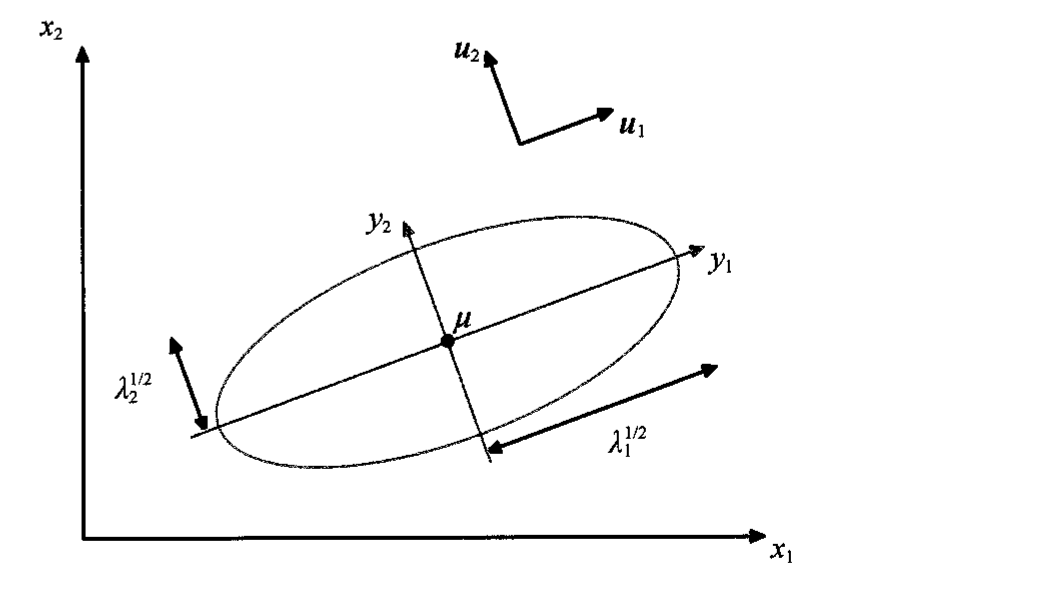
\includegraphics[width=0.78\textwidth]{ch03-fig3-3-gauss-ellipse.png}
  \caption{红色曲线表示 Gauss 分布在二维空间 $\boldsymbol{x}=(x_1,x_2)$ 中具有恒定概率密度的椭圆面，椭圆面上的密度是其在 $\boldsymbol{x}=\boldsymbol{\mu}$ 处取值的 $\exp(-1/2)$ 倍。椭圆的轴由协方差矩阵的特征向量 $\boldsymbol{u}_i$ 定义，具有相应的特征值 $\lambda_i$。}
  \label{figure:ch03-Gauss椭球}
\end{figure}

为了给出良定的 Gauss 分布，需要保证协方差矩阵的所有特征值 $\lambda_i$ 均严格为正，否则分布就无法被正确归一化。特征值全部严格为正的矩阵是正定的（参见\cref{chapter:ch16-连续潜变量}）。在讨论隐变量模型时，我们将遇到 Gauss 分布的一个或多个特征值为零的情形。在这种情况下，分布是奇异的且限制在一个更低维的子空间中。如果所有的特征值非负，则称这样的协方差矩阵为半正定的。

考虑 Gauss 分布在由 $y_i$ 定义的新坐标系下的形式。为了从 $\boldsymbol{x}$ 坐标系转换到 $\boldsymbol{y}$ 坐标系，我们使用了 Jacobi 矩阵 $\boldsymbol{J}$，其元素由下式给出：
\begin{align}
J_{ij}=\frac{\partial x_i}{\partial y_j}=U_{ji},
\label{align:ch03-Jacobi矩阵}
\end{align}
其中 $U_{ji}$ 是矩阵 $\boldsymbol{U}^{\mathsf{T}}$ 中的元素。运用矩阵 $\boldsymbol{U}$ 的正交性质，可以得到 Jacobi 矩阵行列式的平方为
\begin{align}
\lvert\boldsymbol{J}\rvert^{2}=\lvert\boldsymbol{U}^{\mathsf{T}}\rvert^{2}=\lvert\boldsymbol{U}^{\mathsf{T}}\rvert\,\lvert\boldsymbol{U}\rvert=\lvert\boldsymbol{U}^{\mathsf{T}}\boldsymbol{U}\rvert=\lvert\boldsymbol{I}\rvert=1,
\label{align:ch03-Jacobi行列式}
\end{align}
从而有 $\lvert\boldsymbol{J}\rvert=1$。同样，协方差矩阵的行列式 $\lvert\boldsymbol{\Sigma}\rvert$ 可以写成特征值的积，于是有
\begin{align}
\lvert\boldsymbol{\Sigma}\rvert^{1/2}=\prod_{j=1}^{D}\lambda_{j}^{1/2}.
\label{align:ch03-协方差行列式}
\end{align}
因此，在 $y_i$ 的坐标系下，Gauss 分布有如下形式：
\begin{align}
p(\boldsymbol{y})=p(\boldsymbol{x})\lvert\boldsymbol{J}\rvert=\prod_{j=1}^{D}\frac{1}{(2\pi\lambda_{j})^{1/2}}\exp\left\{-\frac{y_{j}^{2}}{2\lambda_{j}}\right\}.
\label{align:ch03-旋转Gauss积}
\end{align}

\begin{proposition}[旋转坐标下的 Gauss 密度]\label{proposition:ch03-旋转Gauss}
在\eqref{align:ch03-旋转矩阵}定义的坐标变换 $\boldsymbol{y}=\boldsymbol{U}(\boldsymbol{x}-\boldsymbol{\mu})$ 下，多元 Gauss 密度\eqref{align:ch03-多元Gauss}化为\eqref{align:ch03-旋转Gauss积}，即 $D$ 个相互独立的一元 Gauss 密度的乘积，其第 $j$ 个因子的均值为 $0$、方差为 $\lambda_j$。从而
\begin{align}
\int p(\boldsymbol{y})\,\mathrm{d}\boldsymbol{y}=\prod_{j=1}^{D}\int_{-\infty}^{\infty}\frac{1}{(2\pi\lambda_{j})^{1/2}}\exp\left\{-\frac{y_{j}^{2}}{2\lambda_{j}}\right\}\mathrm{d}y_{j}=1.
\label{align:ch03-Gauss归一验证}
\end{align}
\end{proposition}
\begin{proof}
（重构新增）把\eqref{align:ch03-二次型对角}与\eqref{align:ch03-协方差行列式}代入\eqref{align:ch03-多元Gauss}，并乘以 Jacobi 行列式 $\lvert\boldsymbol{J}\rvert=1$（由\eqref{align:ch03-Jacobi行列式}），即得
\begin{align*}
p(\boldsymbol{y})=\frac{1}{(2\pi)^{D/2}\prod_j\lambda_j^{1/2}}\prod_{j=1}^{D}\exp\left\{-\frac{y_j^{2}}{2\lambda_j}\right\}=\prod_{j=1}^{D}\frac{1}{(2\pi\lambda_j)^{1/2}}\exp\left\{-\frac{y_j^{2}}{2\lambda_j}\right\},
\end{align*}
这就是\eqref{align:ch03-旋转Gauss积}。

对\eqref{align:ch03-旋转Gauss积}积分。由于被积函数是乘积形式且积分变量可分离，
\begin{align*}
\int p(\boldsymbol{y})\,\mathrm{d}\boldsymbol{y}=\prod_{j=1}^{D}\int_{-\infty}^{\infty}\frac{1}{(2\pi\lambda_j)^{1/2}}\exp\left\{-\frac{y_j^{2}}{2\lambda_j}\right\}\mathrm{d}y_j.
\end{align*}
每个因子都是一元 Gauss 密度在 $\mathbb{R}$ 上的积分，由\cref{align:ch02-单变量Gauss}之后给出的归一化结论（一元 Gauss 密度的归一性），其值为 $1$。故乘积为 $1$，即\eqref{align:ch03-Gauss归一验证}，从而验证了多元 Gauss 分布\eqref{align:ch03-多元Gauss}确实是归一化的。
\end{proof}

% SUPPLEMENT: parent=proposition:ch03-旋转Gauss; kind=motivation; location=紧随其后的 remark（重构新增）
\begin{remark}（重构新增）
这条结论是本节的技术核心：它说明多元 Gauss 分布在“特征向量坐标系”下就是 $D$ 个独立的一元 Gauss 分布之积。由此立刻得到两个推论：其一，归一化可以逐因子验证，从而\eqref{align:ch03-多元Gauss}的系数 $(2\pi)^{-D/2}\lvert\boldsymbol{\Sigma}\rvert^{-1/2}$ 是正确的；其二，$\boldsymbol{y}$ 的各分量相互独立，而 $\boldsymbol{x}=\boldsymbol{U}^{\mathsf{T}}\boldsymbol{y}+\boldsymbol{\mu}$ 的分量一般并不独立——相关性完全由 $\boldsymbol{U}$ 的非对角结构承载。

条件 $\lambda_j>0$ 在证明中通过 $\prod_j\lambda_j^{1/2}$ 与 $1/\lambda_j$ 两处使用：若某个 $\lambda_j=0$，相应的因子不再是可积的一元 Gauss 密度，\eqref{align:ch03-Gauss归一验证}失效，这正是“奇异 Gauss 分布不能归一化”的解析表述。
\end{remark}

\subsection{矩}\label{subsection:ch03-矩}

下面考虑 Gauss 分布的矩，并给出对参数 $\boldsymbol{\mu}$ 和 $\boldsymbol{\Sigma}$ 的一种解释。$\boldsymbol{x}$ 在 Gauss 分布下的期望由下式给出：
\begin{align}
\mathbb{E}[\boldsymbol{x}]=\frac{1}{(2\pi)^{D/2}\lvert\boldsymbol{\Sigma}\rvert^{1/2}}\int\exp\left\{-\frac{1}{2}(\boldsymbol{x}-\boldsymbol{\mu})^{\mathsf{T}}\boldsymbol{\Sigma}^{-1}(\boldsymbol{x}-\boldsymbol{\mu})\right\}\boldsymbol{x}\,\mathrm{d}\boldsymbol{x}
=\frac{1}{(2\pi)^{D/2}\lvert\boldsymbol{\Sigma}\rvert^{1/2}}\int\exp\left\{-\frac{1}{2}\boldsymbol{z}^{\mathsf{T}}\boldsymbol{\Sigma}^{-1}\boldsymbol{z}\right\}(\boldsymbol{z}+\boldsymbol{\mu})\,\mathrm{d}\boldsymbol{z},
\label{align:ch03-Gauss均值期望}
\end{align}
这里进行了变量替换 $\boldsymbol{z}=\boldsymbol{x}-\boldsymbol{\mu}$。注意指数项是 $\boldsymbol{z}$ 的偶函数，且由于是在 $(-\infty,\infty)$ 上求积分，因此 $(\boldsymbol{z}+\boldsymbol{\mu})$ 中的 $\boldsymbol{z}$ 将由于对称性而消去。于是有
\begin{align}
\mathbb{E}[\boldsymbol{x}]=\boldsymbol{\mu}.
\label{align:ch03-Gauss均值}
\end{align}

接下来考虑 Gauss 分布的二阶矩。在单变量的情形下，我们知道二阶矩由 $\mathbb{E}[x^{2}]$ 给出。对于多变量的 Gauss 分布，存在由 $\mathbb{E}[x_i x_j]$ 给出的 $D^{2}$ 个二阶矩。我们可以将它们组合成矩阵 $\mathbb{E}[\boldsymbol{x}\boldsymbol{x}^{\mathsf{T}}]$，该矩阵可以写作
\begin{align}
\mathbb{E}[\boldsymbol{x}\boldsymbol{x}^{\mathsf{T}}]=\frac{1}{(2\pi)^{D/2}\lvert\boldsymbol{\Sigma}\rvert^{1/2}}\int\exp\left\{-\frac{1}{2}(\boldsymbol{x}-\boldsymbol{\mu})^{\mathsf{T}}\boldsymbol{\Sigma}^{-1}(\boldsymbol{x}-\boldsymbol{\mu})\right\}\boldsymbol{x}\boldsymbol{x}^{\mathsf{T}}\,\mathrm{d}\boldsymbol{x}.
\label{align:ch03-二阶矩积分}
\end{align}
这里再一次进行了变量替换 $\boldsymbol{z}=\boldsymbol{x}-\boldsymbol{\mu}$。注意交叉项中涉及的 $\boldsymbol{\mu}\boldsymbol{z}^{\mathsf{T}}$ 和 $\boldsymbol{z}\boldsymbol{\mu}^{\mathsf{T}}$ 也会由于对称性而消去。项 $\boldsymbol{\mu}\boldsymbol{\mu}^{\mathsf{T}}$ 取常值，因此可以拿到积分号之外。由于 Gauss 分布是归一化的，因此它是单位矩阵。可以再一次利用\eqref{align:ch03-特征方程}给出的协方差矩阵的特征向量扩展，以及特征向量集的完备性，写出
\begin{align}
\mathbb{E}[\boldsymbol{x}\boldsymbol{x}^{\mathsf{T}}]=\frac{1}{(2\pi)^{D/2}\lvert\boldsymbol{\Sigma}\rvert^{1/2}}\int\exp\left\{-\frac{1}{2}\boldsymbol{z}^{\mathsf{T}}\boldsymbol{\Sigma}^{-1}\boldsymbol{z}\right\}\bigl(\boldsymbol{z}\boldsymbol{z}^{\mathsf{T}}+\boldsymbol{\mu}\boldsymbol{\mu}^{\mathsf{T}}\bigr)\,\mathrm{d}\boldsymbol{z},
\label{align:ch03-二阶矩展开}
\end{align}
其中 $\boldsymbol{z}=\sum_{i}y_{i}\boldsymbol{u}_{i}$，从而有
\begin{align}
\mathbb{E}[\boldsymbol{x}\boldsymbol{x}^{\mathsf{T}}]=\boldsymbol{\mu}\boldsymbol{\mu}^{\mathsf{T}}+\sum_{i,j}\boldsymbol{u}_{i}\boldsymbol{u}_{j}^{\mathsf{T}}\int\frac{1}{(2\pi)^{D/2}\lvert\boldsymbol{\Sigma}\rvert^{1/2}}\exp\left\{-\frac{1}{2}\sum_{k}\frac{y_{k}^{2}}{\lambda_{k}}\right\}y_{i}y_{j}\,\mathrm{d}\boldsymbol{y}.
\label{align:ch03-二阶矩谱}
\end{align}
这里用到了特征向量等式\eqref{align:ch03-特征方程}，以及对称性导致中间行除 $i=j$ 之外的积分项消去的事实。\eqref{align:ch03-二阶矩谱}的最后一行用到了\cref{align:ch03-旋转Gauss积}和\cref{align:ch03-协方差行列式}的结果，并结合了\eqref{align:ch03-协方差谱分解}。于是有
\begin{align}
\mathbb{E}[\boldsymbol{x}\boldsymbol{x}^{\mathsf{T}}]=\boldsymbol{\mu}\boldsymbol{\mu}^{\mathsf{T}}+\boldsymbol{\Sigma}.
\label{align:ch03-二阶矩}
\end{align}

\begin{proposition}[多元 Gauss 分布的一阶矩与二阶矩]\label{proposition:ch03-Gauss矩}
设 $\boldsymbol{x}\sim\mathcal{N}(\boldsymbol{x}\mid\boldsymbol{\mu},\boldsymbol{\Sigma})$，$\boldsymbol{\Sigma}$ 对称正定。则
\begin{align*}
\mathbb{E}[\boldsymbol{x}]=\boldsymbol{\mu},\qquad \mathbb{E}[\boldsymbol{x}\boldsymbol{x}^{\mathsf{T}}]=\boldsymbol{\mu}\boldsymbol{\mu}^{\mathsf{T}}+\boldsymbol{\Sigma}.
\end{align*}
\end{proposition}
\begin{proof}
（重构新增）第一式的推导即\eqref{align:ch03-Gauss均值期望}至\eqref{align:ch03-Gauss均值}：作变量替换 $\boldsymbol{z}=\boldsymbol{x}-\boldsymbol{\mu}$ 后，被积函数 $\exp\{-\frac12\boldsymbol{z}^{\mathsf{T}}\boldsymbol{\Sigma}^{-1}\boldsymbol{z}\}\boldsymbol{z}$ 关于 $\boldsymbol{z}$ 是奇函数，而积分区域 $\mathbb{R}^{D}$ 关于原点对称，故这部分积分为零；剩下 $\boldsymbol{\mu}$ 乘以归一化积分，其值为 $\boldsymbol{\mu}$。

第二式：由\eqref{align:ch03-旋转矩阵}，$\boldsymbol{z}=\boldsymbol{U}^{\mathsf{T}}\boldsymbol{y}$，即 $\boldsymbol{z}=\sum_i y_i\boldsymbol{u}_i$，其中 $\boldsymbol{y}$ 的各分量相互独立，且由\eqref{align:ch03-旋转Gauss积}，$\mathbb{E}[y_i]=0$、$\mathbb{E}[y_i^{2}]=\lambda_i$。于是
\begin{align*}
\mathbb{E}[\boldsymbol{z}\boldsymbol{z}^{\mathsf{T}}]=\sum_{i,j}\boldsymbol{u}_i\boldsymbol{u}_j^{\mathsf{T}}\mathbb{E}[y_iy_j]=\sum_{i}\lambda_i\boldsymbol{u}_i\boldsymbol{u}_i^{\mathsf{T}}=\boldsymbol{\Sigma},
\end{align*}
其中第二步用到独立性（$i\neq j$ 时 $\mathbb{E}[y_iy_j]=\mathbb{E}[y_i]\mathbb{E}[y_j]=0$），最后一步用到\eqref{align:ch03-协方差谱分解}。再由 $\boldsymbol{x}=\boldsymbol{z}+\boldsymbol{\mu}$ 展开 $\mathbb{E}[\boldsymbol{x}\boldsymbol{x}^{\mathsf{T}}]=\mathbb{E}[\boldsymbol{z}\boldsymbol{z}^{\mathsf{T}}]+\boldsymbol{\mu}\mathbb{E}[\boldsymbol{z}^{\mathsf{T}}]+\mathbb{E}[\boldsymbol{z}]\boldsymbol{\mu}^{\mathsf{T}}+\boldsymbol{\mu}\boldsymbol{\mu}^{\mathsf{T}}$，并利用 $\mathbb{E}[\boldsymbol{z}]=0$，即得\eqref{align:ch03-二阶矩}。
\end{proof}

% SUPPLEMENT: parent=proposition:ch03-Gauss矩; kind=motivation; location=紧随其后的 remark（重构新增）
\begin{remark}（重构新增）
这两条结论给出了“$\boldsymbol{\mu}$ 与 $\boldsymbol{\Sigma}$ 就是均值与协方差”这一说法：$\mathbb{E}[\boldsymbol{x}]=\boldsymbol{\mu}$ 说明第一个参数是位置参数，$\mathbb{E}[\boldsymbol{x}\boldsymbol{x}^{\mathsf{T}}]=\boldsymbol{\mu}\boldsymbol{\mu}^{\mathsf{T}}+\boldsymbol{\Sigma}$ 说明第二个参数承担了扣除均值后的全部二阶波动。

推导中两次用到“对称性消去”：一次是对奇函数在对称区域上的积分为零，一次是 $i\neq j$ 时 $y_i$ 与 $y_j$ 独立而使交叉项的期望为零。前者只依赖于积分区域的对称性与被积函数的奇偶性，后者依赖\eqref{align:ch03-旋转Gauss积}给出的独立性；若 $\boldsymbol{\Sigma}$ 不是正定的（例如奇异），这些积分未必存在，结论也就不再成立。
\end{remark}

在定义单个随机变量的方差时，我们在计算二阶矩之前减去了均值。类似地，在多元的情形中，我们再次减去均值，从而将随机变量 $\boldsymbol{x}$ 的协方差定义为
\begin{align}
\mathrm{cov}[\boldsymbol{x}]=\mathbb{E}\left[(\boldsymbol{x}-\mathbb{E}[\boldsymbol{x}])(\boldsymbol{x}-\mathbb{E}[\boldsymbol{x}])^{\mathsf{T}}\right].
\label{align:ch03-协方差定义}
\end{align}

\begin{definition}[随机向量的协方差矩阵]\label{definition:ch03-协方差矩阵}
设 $\boldsymbol{x}$ 为 $D$ 维随机向量且其二阶矩有限，则称由\eqref{align:ch03-协方差定义}定义的 $D\times D$ 矩阵为 $\boldsymbol{x}$ 的协方差矩阵。其 $(i,j)$ 元素为 $\mathrm{cov}[x_i,x_j]=\mathbb{E}[(x_i-\mathbb{E}[x_i])(x_j-\mathbb{E}[x_j])]$。
\end{definition}

% SUPPLEMENT: parent=definition:ch03-协方差矩阵; kind=motivation; location=紧随其后的 remark（重构新增）
\begin{remark}（重构新增）
把方差推广为矩阵，是为了同时记录各分量的波动（对角线）与分量之间的线性相关（非对角线）。由定义立即可见 $\mathrm{cov}[\boldsymbol{x}]$ 是对称矩阵，且对任意实向量 $\boldsymbol{a}$ 有 $\boldsymbol{a}^{\mathsf{T}}\mathrm{cov}[\boldsymbol{x}]\boldsymbol{a}=\mathrm{var}[\boldsymbol{a}^{\mathsf{T}}\boldsymbol{x}]\geqslant0$，因此协方差矩阵总是半正定的；只有当某个线性组合 $\boldsymbol{a}^{\mathsf{T}}\boldsymbol{x}$ 几乎必然为常数时才是奇异的。

定义要求二阶矩有限，否则期望不存在，协方差无从谈起。这一条件在 Gauss 分布情形由 $\boldsymbol{\Sigma}$ 正定自动满足。
\end{remark}

对于特定的 Gauss 分布的情形，我们可以利用 $\mathbb{E}[\boldsymbol{x}]=\boldsymbol{\mu}$ 并结合\eqref{align:ch03-二阶矩}，得到
\begin{align}
\mathrm{cov}[\boldsymbol{x}]=\boldsymbol{\Sigma}.
\label{align:ch03-Gauss协方差}
\end{align}

\begin{proposition}[Gauss 分布的协方差]\label{proposition:ch03-Gauss协方差}
设 $\boldsymbol{x}\sim\mathcal{N}(\boldsymbol{x}\mid\boldsymbol{\mu},\boldsymbol{\Sigma})$，则 $\mathrm{cov}[\boldsymbol{x}]=\boldsymbol{\Sigma}$。
\end{proposition}
\begin{proof}
（重构新增）由\eqref{align:ch03-协方差定义}与期望的线性性，
\begin{align*}
\mathrm{cov}[\boldsymbol{x}]=\mathbb{E}[\boldsymbol{x}\boldsymbol{x}^{\mathsf{T}}]-\mathbb{E}[\boldsymbol{x}]\,\mathbb{E}[\boldsymbol{x}]^{\mathsf{T}}=\bigl(\boldsymbol{\mu}\boldsymbol{\mu}^{\mathsf{T}}+\boldsymbol{\Sigma}\bigr)-\boldsymbol{\mu}\boldsymbol{\mu}^{\mathsf{T}}=\boldsymbol{\Sigma},
\end{align*}
其中第二个等号用到\eqref{align:ch03-二阶矩}与\eqref{align:ch03-Gauss均值}。
\end{proof}

% SUPPLEMENT: parent=proposition:ch03-Gauss协方差; kind=motivation; location=紧随其后的 remark（重构新增）
\begin{remark}（重构新增）
由于参数矩阵 $\boldsymbol{\Sigma}$ 决定了 Gauss 分布下 $\boldsymbol{x}$ 的协方差，因此我们称其为协方差矩阵。这条结论把\eqref{align:ch03-多元Gauss}中的 $\boldsymbol{\Sigma}$ 从“指数里的一个矩阵”提升为“可解释的统计量”，从而使最大似然估计（\cref{subsection:ch03-最大似然}）有了明确的估计目标。

注意证明只用到一阶、二阶矩，因此它对任意均值和协方差为 $\boldsymbol{\mu},\boldsymbol{\Sigma}$ 的分布都给出“二阶矩形式”；反过来，Gauss 分布的特殊性在于它是唯一由 $\boldsymbol{\mu}$ 与 $\boldsymbol{\Sigma}$ 完全确定的分布（见\cref{exercise:ch03-08}的最大熵刻画）。
\end{remark}

\subsection{局限性}\label{subsection:ch03-局限性}

尽管 Gauss 分布\eqref{align:ch03-多元Gauss}经常用作简单的密度模型，但它也存在一些明显的局限性。考虑分布中自由参数的数量：一个常规的对称协方差矩阵 $\boldsymbol{\Sigma}$ 含有 $D(D+1)/2$ 个独立的参数（见\cref{exercise:ch03-15}），$\boldsymbol{\mu}$ 中还另外存在 $D$ 个独立的参数，因此总共有 $D(D+3)/2$ 个参数。对于较大的 $D$，参数量按 $D$ 的平方增长，对较大矩阵的操作和取逆计算代价巨大。

解决这个问题的一种方法是使用协方差矩阵的受限形式。考虑到协方差矩阵是对角的，$\boldsymbol{\Sigma}=\mathrm{diag}(\sigma_i^{2})$，因此密度模型中总共有 $2D$ 个独立参数。相应的概率密度等值线由轴对齐的椭球体给出。我们可以进一步将协方差矩阵限制为与单位矩阵成正比，$\boldsymbol{\Sigma}=\sigma^{2}\boldsymbol{I}$，即所谓各向同性的（isotropic）协方差，这时模型中有 $D+1$ 个独立参数，且概率密度等值线是一个球面。常规协方差矩阵、对角协方差矩阵和各向同性协方差矩阵这 3 种情形如\cref{figure:ch03-协方差等值线}所示。遗憾的是，虽然这些方法限制了分布中的自由度，并使协方差矩阵的求逆变得更快，但它们也极大限制了概率密度的形式，并限制了模型从数据中捕获有趣相关性的能力。

\begin{figure}[htbp]
  \centering
  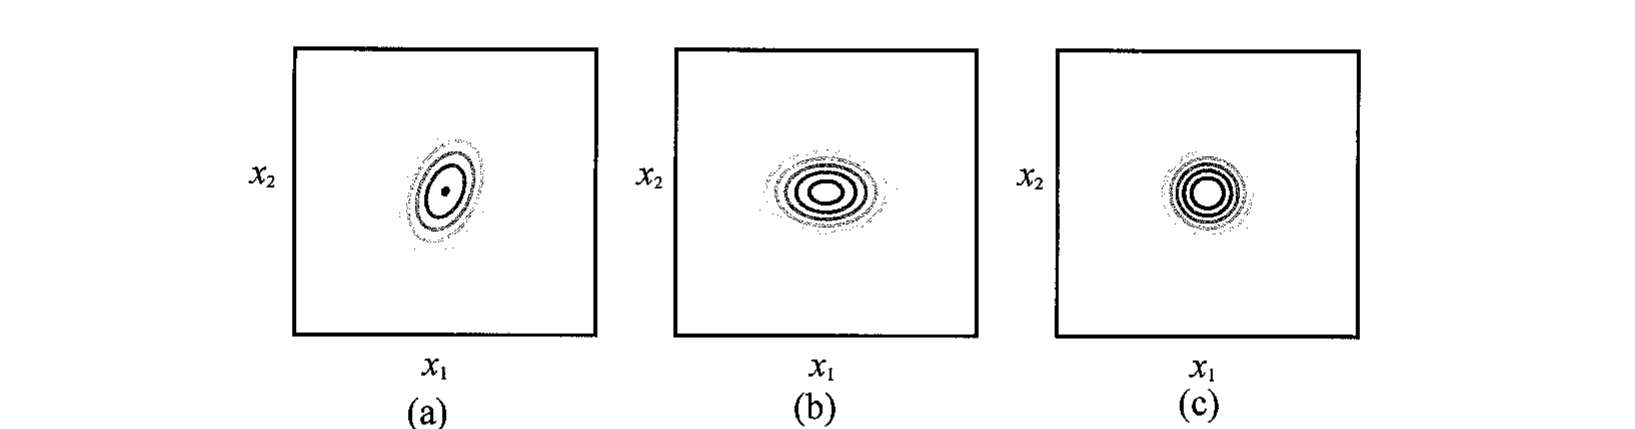
\includegraphics[width=0.92\textwidth]{ch03-fig3-4-cov-contours.png}
  \caption{二维 Gauss 分布的概率密度等值线，其中协方差矩阵为：(a)~常规协方差矩阵；(b)~对角协方差矩阵，在这种情况下，椭圆等值线与坐标轴对齐；(c)~各向同性协方差矩阵，与单位矩阵成正比，在这种情况下，等值线是同心圆。}
  \label{figure:ch03-协方差等值线}
\end{figure}

Gauss 分布的另一个局限性是，它本质上是单峰的（即具有单个最大值），因此无法为多峰分布提供良好的近似。Gauss 分布既存在由于具有太多参数而过于灵活的问题，又存在所能表示的分布太过局限的问题。稍后我们将看到，引入潜变量（也称隐变量或无法观测的变量）可以同时解决上述问题。特别地，通过引入离散潜变量实现 Gauss 混合，可以获得一大类多峰分布（参见\cref{subsection:ch03-Gauss混合}）。同样，连续潜变量的引入将使模型可以独立于数据空间的维度 $D$，控制自由参数的数量，同时仍然允许模型捕获数据集中的主要相关性（参见\cref{chapter:ch16-连续潜变量}）。

\begin{remark}（重构新增）
这一小节指出了 Gauss 分布的“两难”：完整协方差有 $D(D+3)/2$ 个参数，随 $D$ 二次增长，在高维时既难以估计（需要远多于参数个数的样本）又难以计算（求逆为 $O(D^{3})$）；而对角或各向同性的限制虽然把参数降到 $O(D)$，却丢掉了分量之间的相关性，等值线只能是轴对齐椭球或球面。\cref{figure:ch03-协方差等值线}的三个面板正是这三种情形的几何对照。

注意“参数多”与“表达力弱”并不矛盾：完整协方差虽然参数多，但仍然是单峰的，无法表示多峰结构；受限协方差参数少，表达力更弱。解决方向不是继续调整协方差的形式，而是改变模型类——这正是下一小节之后引入混合模型的出发点。
\end{remark}

\subsection{条件分布}\label{subsection:ch03-条件分布}

多元 Gauss 分布的一个重要性质是，如果两组变量服从联合 Gauss 分布，那么以其中一组变量为条件的另一组变量的条件分布是 Gauss 分布。同样，其中任意一组变量的边缘分布也是 Gauss 分布。

首先考虑条件分布的情况。假设 $D$ 维向量 $\boldsymbol{x}$ 服从 Gauss 分布 $\mathcal{N}(\boldsymbol{x}\mid\boldsymbol{\mu},\boldsymbol{\Sigma})$，将 $\boldsymbol{x}$ 划分为两个不相交的子集 $\boldsymbol{x}_{a}$ 和 $\boldsymbol{x}_{b}$。在不失一般性的情况下，我们可以取 $\boldsymbol{x}_{a}$ 为前 $M$ 个分量，并取 $\boldsymbol{x}_{b}$ 作为剩余的 $D-M$ 个分量，于是
\begin{align}
\boldsymbol{x}=\begin{pmatrix}\boldsymbol{x}_{a}\\ \boldsymbol{x}_{b}\end{pmatrix}.
\label{align:ch03-分块}
\end{align}
对均值向量 $\boldsymbol{\mu}$ 定义相应的分量：
\begin{align}
\boldsymbol{\mu}=\begin{pmatrix}\boldsymbol{\mu}_{a}\\ \boldsymbol{\mu}_{b}\end{pmatrix}.
\label{align:ch03-分块均值}
\end{align}
对协方差矩阵 $\boldsymbol{\Sigma}$ 也定义相应的分量：
\begin{align}
\boldsymbol{\Sigma}=\begin{pmatrix}\boldsymbol{\Sigma}_{aa} & \boldsymbol{\Sigma}_{ab}\\ \boldsymbol{\Sigma}_{ba} & \boldsymbol{\Sigma}_{bb}\end{pmatrix}.
\label{align:ch03-分块协方差}
\end{align}
注意，协方差矩阵的对称性 $\boldsymbol{\Sigma}^{\mathsf{T}}=\boldsymbol{\Sigma}$ 意味着 $\boldsymbol{\Sigma}_{aa}$ 和 $\boldsymbol{\Sigma}_{bb}$ 也是对称的，且 $\boldsymbol{\Sigma}_{ba}=\boldsymbol{\Sigma}_{ab}^{\mathsf{T}}$。

在许多情况下，使用协方差矩阵的逆矩阵会更方便：
\begin{align}
\boldsymbol{\Lambda}=\boldsymbol{\Sigma}^{-1}.
\label{align:ch03-精度矩阵}
\end{align}

\begin{definition}[精度矩阵]\label{definition:ch03-精度矩阵}
设 $\boldsymbol{\Sigma}$ 为可逆的协方差矩阵，则称其逆矩阵 $\boldsymbol{\Lambda}=\boldsymbol{\Sigma}^{-1}$ 为精度矩阵（precision matrix）。精度矩阵的分量形式为
\begin{align}
\boldsymbol{\Lambda}=\begin{pmatrix}\boldsymbol{\Lambda}_{aa} & \boldsymbol{\Lambda}_{ab}\\ \boldsymbol{\Lambda}_{ba} & \boldsymbol{\Lambda}_{bb}\end{pmatrix}.
\label{align:ch03-精度矩阵分块}
\end{align}
\end{definition}

% SUPPLEMENT: parent=definition:ch03-精度矩阵; kind=motivation; location=紧随其后的 remark（重构新增）
\begin{remark}（重构新增）
引入精度矩阵是为了让某些性质写起来更简单：本节将看到条件分布的均值和协方差用分量精度矩阵表示最简洁，而边缘分布用分量协方差矩阵表示最简洁。直观上，精度矩阵是“方差的倒数”在矩阵情形的推广——精度越大，分布在该方向上越集中。

注意 $\boldsymbol{\Lambda}_{aa}$ 与 $\boldsymbol{\Sigma}_{aa}^{-1}$ 一般并不相等（\cref{exercise:ch03-18}、\cref{exercise:ch03-23}讨论的正是二者的关系）。这是因为求逆会把分块之间的耦合“混合”进来：$\boldsymbol{\Sigma}_{aa}$ 只描述 $\boldsymbol{x}_a$ 自身的波动，而 $\boldsymbol{\Lambda}_{aa}$ 还包含了 $\boldsymbol{x}_a$ 与 $\boldsymbol{x}_b$ 的相关性对条件化的影响。定义中的可逆性要求与 $\boldsymbol{\Sigma}$ 正定一致。
\end{remark}

这对应于向量 $\boldsymbol{x}$ 的分量形式[\eqref{align:ch03-分块}]。因为对称矩阵的逆矩阵也是对称的（见\cref{exercise:ch03-16}），所以 $\boldsymbol{\Lambda}_{aa}$ 和 $\boldsymbol{\Lambda}_{bb}$ 也是对称的，且有 $\boldsymbol{\Lambda}_{ba}=\boldsymbol{\Lambda}_{ab}^{\mathsf{T}}$。这里需要强调的是，$\boldsymbol{\Lambda}_{aa}=\boldsymbol{\Sigma}_{aa}^{-1}$ 不是简单地由 $\boldsymbol{\Sigma}_{aa}$ 的逆矩阵给出。事实上，我们将很快研究分量矩阵的逆矩阵与其分量的逆矩阵之间的关系。

首先找到条件分布 $p(\boldsymbol{x}_{a}\mid\boldsymbol{x}_{b})$ 的表达式。从概率的乘积法则中，我们看到只需要将 $\boldsymbol{x}_{b}$ 固定为观测值，并归一化表达式以获得关于 $\boldsymbol{x}_{a}$ 的有效概率分布，就可以基于联合分布 $p(\boldsymbol{x})=p(\boldsymbol{x}_{a},\boldsymbol{x}_{b})$ 得到条件分布。有别于显式地执行归一化，我们可以通过考虑\eqref{align:ch03-马氏距离}给出的 Gauss 分布指数中的二次形式，然后在计算结束时恢复归一化系数，从而更高效地获得解。如果使用分量式\eqref{align:ch03-分块}、\eqref{align:ch03-分块均值}、\eqref{align:ch03-精度矩阵分块}，则可以得到
\begin{align}
-\frac{1}{2}(\boldsymbol{x}-\boldsymbol{\mu})^{\mathsf{T}}\boldsymbol{\Sigma}^{-1}(\boldsymbol{x}-\boldsymbol{\mu})=
&-\frac{1}{2}(\boldsymbol{x}_{a}-\boldsymbol{\mu}_{a})^{\mathsf{T}}\boldsymbol{\Lambda}_{aa}(\boldsymbol{x}_{a}-\boldsymbol{\mu}_{a})-\frac{1}{2}(\boldsymbol{x}_{a}-\boldsymbol{\mu}_{a})^{\mathsf{T}}\boldsymbol{\Lambda}_{ab}(\boldsymbol{x}_{b}-\boldsymbol{\mu}_{b})\nonumber\\
&-\frac{1}{2}(\boldsymbol{x}_{b}-\boldsymbol{\mu}_{b})^{\mathsf{T}}\boldsymbol{\Lambda}_{ba}(\boldsymbol{x}_{a}-\boldsymbol{\mu}_{a})-\frac{1}{2}(\boldsymbol{x}_{b}-\boldsymbol{\mu}_{b})^{\mathsf{T}}\boldsymbol{\Lambda}_{bb}(\boldsymbol{x}_{b}-\boldsymbol{\mu}_{b}).
\label{align:ch03-分块二次型}
\end{align}
可以看到，作为 $\boldsymbol{x}_{a}$ 的函数，这又是一个二次形式。因此，相应的条件分布 $p(\boldsymbol{x}_{a}\mid\boldsymbol{x}_{b})$ 将是 Gauss 分布。由于这种分布完全由其均值和协方差确定，因此我们的目标是通过检查\eqref{align:ch03-分块二次型}来确定 $p(\boldsymbol{x}_{a}\mid\boldsymbol{x}_{b})$ 的均值和协方差的表达式。

这是一个与 Gauss 分布相关的相当常见的运算示例，有时称为“完全平方”，我们得到了一个定义了 Gauss 分布中指数项的二次形式。我们需要确定相应的均值和协方差。注意，一般 Gauss 分布 $\mathcal{N}(\boldsymbol{x}\mid\boldsymbol{\mu},\boldsymbol{\Sigma})$ 中的指数可以写成
\begin{align}
-\frac{1}{2}(\boldsymbol{x}-\boldsymbol{\mu})^{\mathsf{T}}\boldsymbol{\Sigma}^{-1}(\boldsymbol{x}-\boldsymbol{\mu})=-\frac{1}{2}\boldsymbol{x}^{\mathsf{T}}\boldsymbol{\Sigma}^{-1}\boldsymbol{x}+\boldsymbol{x}^{\mathsf{T}}\boldsymbol{\Sigma}^{-1}\boldsymbol{\mu}+\text{const},
\label{align:ch03-完全平方恒等式}
\end{align}
其中“const”表示独立于 $\boldsymbol{x}$ 的常数项。再利用 $\boldsymbol{\Sigma}$ 的对称性，这些问题就可以得到解决。因此，如果我们采用一般的二次形式，并用\eqref{align:ch03-完全平方恒等式}右侧给出的形式表示它，则可以立即使 $\boldsymbol{x}$ 中二阶项的系数矩阵等于协方差矩阵的逆矩阵 $\boldsymbol{\Sigma}^{-1}$，然后使 $\boldsymbol{x}$ 中线性项的系数等于 $\boldsymbol{\Sigma}^{-1}\boldsymbol{\mu}$，即可得到 $\boldsymbol{\mu}$。

将此过程应用于条件 Gauss 分布 $p(\boldsymbol{x}_{a}\mid\boldsymbol{x}_{b})$，指数中的二次形式由\eqref{align:ch03-分块二次型}给出。分别用 $\boldsymbol{\mu}_{a\mid b}$ 和 $\boldsymbol{\Sigma}_{a\mid b}$ 表示该分布的均值和协方差。考虑式\eqref{align:ch03-分块二次型}对 $\boldsymbol{x}_{a}$ 的函数依赖性，其中 $\boldsymbol{x}_{b}$ 可以视为常数。如果我们挑选出 $\boldsymbol{x}_{a}$ 中的所有二阶项，则得到
\begin{align}
-\frac{1}{2}\boldsymbol{x}_{a}^{\mathsf{T}}\boldsymbol{\Lambda}_{aa}\boldsymbol{x}_{a},
\label{align:ch03-条件二阶项}
\end{align}
从中我们可以得出一个结论，$p(\boldsymbol{x}_{a}\mid\boldsymbol{x}_{b})$ 的协方差（逆精度）由下式给出：
\begin{align}
\boldsymbol{\Sigma}_{a\mid b}=\boldsymbol{\Lambda}_{aa}^{-1}.
\label{align:ch03-条件协方差精度}
\end{align}
考虑\eqref{align:ch03-分块二次型}中所有在 $\boldsymbol{x}_{a}$ 中呈线性的项：
\begin{align}
\boldsymbol{x}_{a}^{\mathsf{T}}\bigl\{\boldsymbol{\Lambda}_{aa}\boldsymbol{\mu}_{a}-\boldsymbol{\Lambda}_{ab}(\boldsymbol{x}_{b}-\boldsymbol{\mu}_{b})\bigr\},
\label{align:ch03-条件线性项}
\end{align}
这里用到了表达式 $\boldsymbol{\Lambda}_{ba}^{\mathsf{T}}=\boldsymbol{\Lambda}_{ab}$。根据我们对一般形式[\eqref{align:ch03-完全平方恒等式}]的讨论，该表达式中 $\boldsymbol{x}_{a}$ 的系数必须等于 $\boldsymbol{\Sigma}_{a\mid b}^{-1}\boldsymbol{\mu}_{a\mid b}$，故有
\begin{align}
\boldsymbol{\mu}_{a\mid b}&=\boldsymbol{\Sigma}_{a\mid b}\bigl\{\boldsymbol{\Lambda}_{aa}\boldsymbol{\mu}_{a}-\boldsymbol{\Lambda}_{ab}(\boldsymbol{x}_{b}-\boldsymbol{\mu}_{b})\bigr\}\nonumber\\
&=\boldsymbol{\mu}_{a}-\boldsymbol{\Lambda}_{aa}^{-1}\boldsymbol{\Lambda}_{ab}(\boldsymbol{x}_{b}-\boldsymbol{\mu}_{b}).
\label{align:ch03-条件均值精度}
\end{align}
这里用到了表达式\eqref{align:ch03-条件协方差精度}。

\begin{proposition}[条件 Gauss 分布：精度形式]\label{proposition:ch03-条件Gauss精度}
设 $\boldsymbol{x}\sim\mathcal{N}(\boldsymbol{x}\mid\boldsymbol{\mu},\boldsymbol{\Sigma})$ 并按\eqref{align:ch03-分块}至\eqref{align:ch03-精度矩阵分块}分块。则给定 $\boldsymbol{x}_{b}$ 时 $\boldsymbol{x}_{a}$ 的条件分布为 Gauss 分布，其协方差与均值分别为
\begin{align*}
\boldsymbol{\Sigma}_{a\mid b}=\boldsymbol{\Lambda}_{aa}^{-1},\qquad \boldsymbol{\mu}_{a\mid b}=\boldsymbol{\mu}_{a}-\boldsymbol{\Lambda}_{aa}^{-1}\boldsymbol{\Lambda}_{ab}(\boldsymbol{x}_{b}-\boldsymbol{\mu}_{b}).
\end{align*}
且该条件分布与 $\boldsymbol{x}_{b}$ 的取值无关（协方差不依赖 $\boldsymbol{x}_{b}$）。
\end{proposition}
\begin{proof}
（重构新增）由\eqref{align:ch03-分块二次型}，联合密度的指数（忽略常数 $-1/2$ 与不依赖 $\boldsymbol{x}_a$ 的项）是 $\boldsymbol{x}_{a}$ 的二次函数，故条件密度 $p(\boldsymbol{x}_{a}\mid\boldsymbol{x}_{b})\propto p(\boldsymbol{x}_{a},\boldsymbol{x}_{b})$（把 $\boldsymbol{x}_{b}$ 视为常数）也是 $\boldsymbol{x}_{a}$ 的二次指数形式，即为 Gauss 分布。

将其与\eqref{align:ch03-完全平方恒等式}对照： $\boldsymbol{x}_{a}$ 的二阶项系数矩阵为 $\boldsymbol{\Lambda}_{aa}$，故条件分布的精度矩阵为 $\boldsymbol{\Lambda}_{aa}$，即协方差为 $\boldsymbol{\Lambda}_{aa}^{-1}$，这就是\eqref{align:ch03-条件协方差精度}。 $\boldsymbol{x}_{a}$ 的线性项系数由\eqref{align:ch03-条件线性项}给出，为 $\boldsymbol{\Lambda}_{aa}\boldsymbol{\mu}_{a}-\boldsymbol{\Lambda}_{ab}(\boldsymbol{x}_{b}-\boldsymbol{\mu}_{b})$，它必须等于 $\boldsymbol{\Sigma}_{a\mid b}^{-1}\boldsymbol{\mu}_{a\mid b}=\boldsymbol{\Lambda}_{aa}\boldsymbol{\mu}_{a\mid b}$，两边左乘 $\boldsymbol{\Lambda}_{aa}^{-1}$ 即得\eqref{align:ch03-条件均值精度}。由于指数中只出现 $\boldsymbol{x}_{a}$ 的二次项与线性项，条件密度必定是归一化的 Gauss 密度，其均值与协方差如上。
\end{proof}

% SUPPLEMENT: parent=proposition:ch03-条件Gauss精度; kind=motivation; location=紧随其后的 remark（重构新增）
\begin{remark}（重构新增）
“完全平方”是处理 Gauss 分布二次型的标准技巧：只要把指数写成 $-\frac12\boldsymbol{x}^{\mathsf{T}}\boldsymbol{A}\boldsymbol{x}+\boldsymbol{x}^{\mathsf{T}}\boldsymbol{b}+\text{const}$ 的形式，就能立刻读出协方差 $\boldsymbol{A}^{-1}$ 与均值 $\boldsymbol{A}^{-1}\boldsymbol{b}$。这里 $\boldsymbol{A}=\boldsymbol{\Lambda}_{aa}$、$\boldsymbol{b}=\boldsymbol{\Lambda}_{aa}\boldsymbol{\mu}_{a}-\boldsymbol{\Lambda}_{ab}(\boldsymbol{x}_{b}-\boldsymbol{\mu}_{b})$。

条件分布的协方差 $\boldsymbol{\Lambda}_{aa}^{-1}$ 与 $\boldsymbol{x}_{b}$ 无关，这一事实非常重要：它说明“观测到 $\boldsymbol{x}_b$ 只移动条件分布的均值，不改变其形状”。均值是 $\boldsymbol{x}_{b}$ 的线性函数，这正是线性-Gauss 结构的来源。注意这里用到 $\boldsymbol{\Lambda}_{aa}$ 可逆，而它由 $\boldsymbol{\Sigma}$ 正定保证。
\end{remark}

式\eqref{align:ch03-条件协方差精度}和式\eqref{align:ch03-条件均值精度}给出的结果可以用原始联合分布 $p(\boldsymbol{x}_{a},\boldsymbol{x}_{b})$ 的分量精度矩阵来表示。也可以用相应的分量协方差矩阵来表示这些结果。为此，对分量矩阵的逆矩阵使用以下恒等式（见\cref{exercise:ch03-18}）：
\begin{align}
\begin{pmatrix}\boldsymbol{A} & \boldsymbol{B}\\ \boldsymbol{C} & \boldsymbol{D}\end{pmatrix}^{-1}=\begin{pmatrix}\boldsymbol{M} & -\boldsymbol{M}\boldsymbol{B}\boldsymbol{D}^{-1}\\ -\boldsymbol{D}^{-1}\boldsymbol{C}\boldsymbol{M} & \boldsymbol{D}^{-1}+\boldsymbol{D}^{-1}\boldsymbol{C}\boldsymbol{M}\boldsymbol{B}\boldsymbol{D}^{-1}\end{pmatrix},
\label{align:ch03-分块逆}
\end{align}
其中
\begin{align}
\boldsymbol{M}=(\boldsymbol{A}-\boldsymbol{B}\boldsymbol{D}^{-1}\boldsymbol{C})^{-1}.
\label{align:ch03-舒尔补}
\end{align}
量 $\boldsymbol{M}^{-1}$ 称为\eqref{align:ch03-分块逆}左侧矩阵相对于子矩阵 $\boldsymbol{D}$ 的 Schur 补（Schur complement）。利用定义
\begin{align}
\begin{pmatrix}\boldsymbol{\Sigma}_{aa} & \boldsymbol{\Sigma}_{ab}\\ \boldsymbol{\Sigma}_{ba} & \boldsymbol{\Sigma}_{bb}\end{pmatrix}^{-1}=\begin{pmatrix}\boldsymbol{\Lambda}_{aa} & \boldsymbol{\Lambda}_{ab}\\ \boldsymbol{\Lambda}_{ba} & \boldsymbol{\Lambda}_{bb}\end{pmatrix},
\label{align:ch03-分块逆对应}
\end{align}
并使用\eqref{align:ch03-分块逆}，有
\begin{align}
\boldsymbol{\Lambda}_{aa}=\bigl(\boldsymbol{\Sigma}_{aa}-\boldsymbol{\Sigma}_{ab}\boldsymbol{\Sigma}_{bb}^{-1}\boldsymbol{\Sigma}_{ba}\bigr)^{-1},
\label{align:ch03-精度分块aa}
\end{align}
\begin{align}
\boldsymbol{\Lambda}_{ab}=-\bigl(\boldsymbol{\Sigma}_{aa}-\boldsymbol{\Sigma}_{ab}\boldsymbol{\Sigma}_{bb}^{-1}\boldsymbol{\Sigma}_{ba}\bigr)^{-1}\boldsymbol{\Sigma}_{ab}\boldsymbol{\Sigma}_{bb}^{-1}.
\label{align:ch03-精度分块ab}
\end{align}
条件分布 $p(\boldsymbol{x}_{a}\mid\boldsymbol{x}_{b})$ 的均值和协方差可以通过以下表达式获得：
\begin{align}
\boldsymbol{\mu}_{a\mid b}=\boldsymbol{\mu}_{a}+\boldsymbol{\Sigma}_{ab}\boldsymbol{\Sigma}_{bb}^{-1}(\boldsymbol{x}_{b}-\boldsymbol{\mu}_{b}),
\label{align:ch03-条件均值}
\end{align}
\begin{align}
\boldsymbol{\Sigma}_{a\mid b}=\boldsymbol{\Sigma}_{aa}-\boldsymbol{\Sigma}_{ab}\boldsymbol{\Sigma}_{bb}^{-1}\boldsymbol{\Sigma}_{ba}.
\label{align:ch03-条件协方差}
\end{align}
比较\eqref{align:ch03-条件协方差精度}和\eqref{align:ch03-条件协方差}，可以看到条件分布 $p(\boldsymbol{x}_{a}\mid\boldsymbol{x}_{b})$ 在用分量精度矩阵表示时，比用分量协方差矩阵表示时更简单。

\begin{proposition}[条件 Gauss 分布：协方差形式]\label{proposition:ch03-条件Gauss协方差}
在\cref{proposition:ch03-条件Gauss精度}的设定下，条件分布 $p(\boldsymbol{x}_{a}\mid\boldsymbol{x}_{b})$ 的均值与协方差亦可写成\eqref{align:ch03-条件均值}与\eqref{align:ch03-条件协方差}，即
\begin{align*}
\boldsymbol{\mu}_{a\mid b}=\boldsymbol{\mu}_{a}+\boldsymbol{\Sigma}_{ab}\boldsymbol{\Sigma}_{bb}^{-1}(\boldsymbol{x}_{b}-\boldsymbol{\mu}_{b}),\qquad \boldsymbol{\Sigma}_{a\mid b}=\boldsymbol{\Sigma}_{aa}-\boldsymbol{\Sigma}_{ab}\boldsymbol{\Sigma}_{bb}^{-1}\boldsymbol{\Sigma}_{ba}.
\end{align*}
\end{proposition}
\begin{proof}
（重构新增）由\eqref{align:ch03-分块逆对应}与\eqref{align:ch03-分块逆}（取 $\boldsymbol{A}=\boldsymbol{\Sigma}_{aa}$，$\boldsymbol{B}=\boldsymbol{\Sigma}_{ab}$，$\boldsymbol{C}=\boldsymbol{\Sigma}_{ba}$，$\boldsymbol{D}=\boldsymbol{\Sigma}_{bb}$），可得\eqref{align:ch03-精度分块aa}与\eqref{align:ch03-精度分块ab}。

由\eqref{align:ch03-条件协方差精度}，$\boldsymbol{\Sigma}_{a\mid b}=\boldsymbol{\Lambda}_{aa}^{-1}$，对\eqref{align:ch03-精度分块aa}取逆即得\eqref{align:ch03-条件协方差}。

由\eqref{align:ch03-条件均值精度}，
\begin{align*}
\boldsymbol{\mu}_{a\mid b}=\boldsymbol{\mu}_{a}-\boldsymbol{\Lambda}_{aa}^{-1}\boldsymbol{\Lambda}_{ab}(\boldsymbol{x}_{b}-\boldsymbol{\mu}_{b}).
\end{align*}
把\eqref{align:ch03-精度分块aa}的逆 $\boldsymbol{\Lambda}_{aa}^{-1}=\boldsymbol{\Sigma}_{aa}-\boldsymbol{\Sigma}_{ab}\boldsymbol{\Sigma}_{bb}^{-1}\boldsymbol{\Sigma}_{ba}$ 与\eqref{align:ch03-精度分块ab}代入，得
\begin{align*}
-\boldsymbol{\Lambda}_{aa}^{-1}\boldsymbol{\Lambda}_{ab}=\bigl(\boldsymbol{\Sigma}_{aa}-\boldsymbol{\Sigma}_{ab}\boldsymbol{\Sigma}_{bb}^{-1}\boldsymbol{\Sigma}_{ba}\bigr)\bigl(\boldsymbol{\Sigma}_{aa}-\boldsymbol{\Sigma}_{ab}\boldsymbol{\Sigma}_{bb}^{-1}\boldsymbol{\Sigma}_{ba}\bigr)^{-1}\boldsymbol{\Sigma}_{ab}\boldsymbol{\Sigma}_{bb}^{-1}=\boldsymbol{\Sigma}_{ab}\boldsymbol{\Sigma}_{bb}^{-1},
\end{align*}
于是 $\boldsymbol{\mu}_{a\mid b}=\boldsymbol{\mu}_{a}+\boldsymbol{\Sigma}_{ab}\boldsymbol{\Sigma}_{bb}^{-1}(\boldsymbol{x}_{b}-\boldsymbol{\mu}_{b})$，即\eqref{align:ch03-条件均值}。
\end{proof}

% SUPPLEMENT: parent=proposition:ch03-条件Gauss协方差; kind=motivation; location=紧随其后的 remark（重构新增）
\begin{remark}（重构新增）
两种写法各有用途：协方差形式\eqref{align:ch03-条件均值}\eqref{align:ch03-条件协方差}只用联合分布的分量协方差矩阵，直观地显示“条件均值是从先验均值出发、沿回归系数 $\boldsymbol{\Sigma}_{ab}\boldsymbol{\Sigma}_{bb}^{-1}$ 修正”；精度形式则说明条件协方差就是 $\boldsymbol{\Lambda}_{aa}^{-1}$，无需计算 Schur 补。

这里出现了两个不同的 Schur 补且互为逆矩阵：$\boldsymbol{\Lambda}_{aa}=(\boldsymbol{\Sigma}_{aa}-\boldsymbol{\Sigma}_{ab}\boldsymbol{\Sigma}_{bb}^{-1}\boldsymbol{\Sigma}_{ba})^{-1}$。证明中两次用到 $\boldsymbol{\Sigma}_{bb}$ 可逆，这由 $\boldsymbol{\Sigma}$ 正定保证（正定矩阵的主子块正定）。若 $\boldsymbol{\Sigma}_{bb}$ 奇异，则 $\boldsymbol{x}_b$ 的分布在某个方向上退化，条件化需要另行处理。
\end{remark}

注意，由\eqref{align:ch03-条件均值}给出的条件分布 $p(\boldsymbol{x}_{a}\mid\boldsymbol{x}_{b})$ 的均值是 $\boldsymbol{x}_{b}$ 的线性函数，而\eqref{align:ch03-条件协方差}给出的协方差与 $\boldsymbol{x}_{b}$ 无关。这是线性-Gauss（linear-Gaussian）模型的一个示例（参见\cref{subsection:ch11-Gauss变量}）。

\begin{definition}[线性-Gauss 模型]\label{definition:ch03-线性Gauss模型}
设 $\boldsymbol{x}$ 与 $\boldsymbol{y}$ 为随机向量。若给定 $\boldsymbol{x}$ 时 $\boldsymbol{y}$ 的条件分布为 Gauss 分布，且其均值是 $\boldsymbol{x}$ 的线性函数、其协方差与 $\boldsymbol{x}$ 无关，即
\begin{align}
p(\boldsymbol{y}\mid\boldsymbol{x})=\mathcal{N}\bigl(\boldsymbol{y}\mid\boldsymbol{A}\boldsymbol{x}+\boldsymbol{b},\boldsymbol{L}^{-1}\bigr),
\label{align:ch03-线性Gauss模型}
\end{align}
则称 $(\boldsymbol{x},\boldsymbol{y})$ 服从线性-Gauss 模型，其中 $\boldsymbol{A},\boldsymbol{b}$ 为控制均值的参数，$\boldsymbol{L}$ 为精度矩阵。
\end{definition}

% SUPPLEMENT: parent=definition:ch03-线性Gauss模型; kind=motivation; location=紧随其后的 remark（重构新增）
\begin{remark}（重构新增）
线性-Gauss 模型之所以重要，是因为它同时具备两个良好性质：条件分布的均值对 $\boldsymbol{x}$ 线性（便于解释为“回归”），协方差不随 $\boldsymbol{x}$ 变化（便于计算）。这两点正是\eqref{align:ch03-条件均值}与\eqref{align:ch03-条件协方差}所显示的结构，因此任何联合 Gauss 分布按分量分块后都自动成为线性-Gauss 模型。

条件 $\boldsymbol{L}$ 为正定（即精度矩阵可逆）保证条件密度良定义；若 $\boldsymbol{A}$ 不是满秩，则 $\boldsymbol{y}$ 的均值只落在 $\boldsymbol{x}$ 的一个线性子空间上，但分布本身仍然良定义。下一小节将看到，线性-Gauss 结构在 Bayes 定理下封闭：先验 Gauss、似然线性-Gauss 时，后验仍是 Gauss（\cref{subsection:ch03-Bayes定理}）。
\end{remark}

\subsection{边缘分布}\label{subsection:ch03-边缘分布}

我们已经看到，如果联合分布 $p(\boldsymbol{x}_{a},\boldsymbol{x}_{b})$ 是 Gauss 分布，则条件分布 $p(\boldsymbol{x}_{a}\mid\boldsymbol{x}_{b})$ 也是 Gauss 分布。现在我们接着讨论由下式给出的边缘分布：
\begin{align}
p(\boldsymbol{x}_{a})=\int p(\boldsymbol{x}_{a},\boldsymbol{x}_{b})\,\mathrm{d}\boldsymbol{x}_{b}.
\label{align:ch03-边缘积分}
\end{align}
正如我们将看到的，它也是 Gauss 分布。与之前相同，我们计算这种分布的策略是关注联合分布指数中的二次形式，从而确定边缘分布 $p(\boldsymbol{x}_{a})$ 的均值和协方差。

联合分布指数中的二次形式可以用\eqref{align:ch03-分块二次型}中的分量精度矩阵来表示。我们的目标是通过积分消去 $\boldsymbol{x}_{b}$，而最容易实现的是首先考虑涉及 $\boldsymbol{x}_{b}$ 的项，然后完全平方以完成积分。通过选出那些涉及 $\boldsymbol{x}_{b}$ 的项，有
\begin{align}
-\frac{1}{2}\boldsymbol{x}_{b}^{\mathsf{T}}\boldsymbol{\Lambda}_{bb}\boldsymbol{x}_{b}+\boldsymbol{x}_{b}^{\mathsf{T}}\boldsymbol{m}=-\frac{1}{2}\bigl(\boldsymbol{x}_{b}-\boldsymbol{\Lambda}_{bb}^{-1}\boldsymbol{m}\bigr)^{\mathsf{T}}\boldsymbol{\Lambda}_{bb}\bigl(\boldsymbol{x}_{b}-\boldsymbol{\Lambda}_{bb}^{-1}\boldsymbol{m}\bigr)+\frac{1}{2}\boldsymbol{m}^{\mathsf{T}}\boldsymbol{\Lambda}_{bb}^{-1}\boldsymbol{m},
\label{align:ch03-边缘完全平方}
\end{align}
其中
\begin{align}
\boldsymbol{m}=\boldsymbol{\Lambda}_{bb}\boldsymbol{\mu}_{b}-\boldsymbol{\Lambda}_{ba}(\boldsymbol{x}_{a}-\boldsymbol{\mu}_{a}).
\label{align:ch03-边缘辅助向量}
\end{align}
可以看到，对 $\boldsymbol{x}_{b}$ 的依赖性已转换为 Gauss 分布的标准二次形式，对应于\eqref{align:ch03-边缘完全平方}右侧的第一项加上一个不依赖于 $\boldsymbol{x}_{b}$（但依赖于 $\boldsymbol{x}_{a}$）的项。因此，当我们取这个二次形式的指数时，可以看到\eqref{align:ch03-边缘积分}所需的对 $\boldsymbol{x}_{b}$ 的积分将采用以下形式：
\begin{align}
\int\exp\left\{-\frac{1}{2}\bigl(\boldsymbol{x}_{b}-\boldsymbol{\Lambda}_{bb}^{-1}\boldsymbol{m}\bigr)^{\mathsf{T}}\boldsymbol{\Lambda}_{bb}\bigl(\boldsymbol{x}_{b}-\boldsymbol{\Lambda}_{bb}^{-1}\boldsymbol{m}\bigr)\right\}\mathrm{d}\boldsymbol{x}_{b}.
\label{align:ch03-边缘积分消去}
\end{align}
这种积分很容易实现，由于该分布是未归一化的 Gauss 分布，因此积分的结果将是归一化系数的倒数。由\eqref{align:ch03-多元Gauss}给出的归一化 Gauss 形式可知，该系数与均值无关，而仅取决于协方差矩阵的行列式。因此，通过计算完全关于 $\boldsymbol{x}_{b}$ 的平方，可以积分消去 $\boldsymbol{x}_{b}$，于是\eqref{align:ch03-边缘完全平方}左侧唯一剩下的依赖于 $\boldsymbol{x}_{a}$ 的项就是\eqref{align:ch03-边缘完全平方}右侧的最后一项，其中 $\boldsymbol{m}$ 由\eqref{align:ch03-边缘辅助向量}给出。将该项与\eqref{align:ch03-分块二次型}中依赖于 $\boldsymbol{x}_{a}$ 的其余项相结合，可以得到
\begin{align}
&\frac{1}{2}\bigl[\boldsymbol{\Lambda}_{bb}\boldsymbol{\mu}_{b}-\boldsymbol{\Lambda}_{ba}(\boldsymbol{x}_{a}-\boldsymbol{\mu}_{a})\bigr]^{\mathsf{T}}\boldsymbol{\Lambda}_{bb}^{-1}\bigl[\boldsymbol{\Lambda}_{bb}\boldsymbol{\mu}_{b}-\boldsymbol{\Lambda}_{ba}(\boldsymbol{x}_{a}-\boldsymbol{\mu}_{a})\bigr]\nonumber\\
&\quad-\frac{1}{2}\boldsymbol{x}_{a}^{\mathsf{T}}\boldsymbol{\Lambda}_{aa}\boldsymbol{x}_{a}+\boldsymbol{x}_{a}^{\mathsf{T}}\bigl(\boldsymbol{\Lambda}_{aa}\boldsymbol{\mu}_{a}+\boldsymbol{\Lambda}_{ab}\boldsymbol{\mu}_{b}\bigr)+\text{const}\nonumber\\
&\quad=-\frac{1}{2}\boldsymbol{x}_{a}^{\mathsf{T}}\bigl(\boldsymbol{\Lambda}_{aa}-\boldsymbol{\Lambda}_{ab}\boldsymbol{\Lambda}_{bb}^{-1}\boldsymbol{\Lambda}_{ba}\bigr)\boldsymbol{x}_{a}+\boldsymbol{x}_{a}^{\mathsf{T}}\bigl(\boldsymbol{\Lambda}_{aa}-\boldsymbol{\Lambda}_{ab}\boldsymbol{\Lambda}_{bb}^{-1}\boldsymbol{\Lambda}_{ba}\bigr)\boldsymbol{\mu}_{a}+\text{const},
\label{align:ch03-边缘二次型}
\end{align}
其中“const”表示独立于 $\boldsymbol{x}_{a}$ 的常数项。同样，通过与\eqref{align:ch03-完全平方恒等式}进行比较，可以看到边缘分布 $p(\boldsymbol{x}_{a})$ 的协方差由下式给出：
\begin{align}
\boldsymbol{\Sigma}_{a}=\bigl(\boldsymbol{\Lambda}_{aa}-\boldsymbol{\Lambda}_{ab}\boldsymbol{\Lambda}_{bb}^{-1}\boldsymbol{\Lambda}_{ba}\bigr)^{-1}.
\label{align:ch03-边缘协方差精度}
\end{align}
均值则由下式给出：
\begin{align}
\boldsymbol{\Sigma}_{a}\bigl(\boldsymbol{\Lambda}_{aa}-\boldsymbol{\Lambda}_{ab}\boldsymbol{\Lambda}_{bb}^{-1}\boldsymbol{\Lambda}_{ba}\bigr)\boldsymbol{\mu}_{a}=\boldsymbol{\mu}_{a}.
\label{align:ch03-边缘均值精度}
\end{align}
这里用到了\eqref{align:ch03-边缘协方差精度}。协方差式\eqref{align:ch03-边缘协方差精度}是用\eqref{align:ch03-精度矩阵分块}给出的分量精度矩阵来表示的。就像我们对条件分布所做的那样，我们可以根据\eqref{align:ch03-分块协方差}给出的协方差矩阵的相应分量来重写它。这些分量矩阵有如下关系：
\begin{align}
\begin{pmatrix}\boldsymbol{\Lambda}_{aa} & \boldsymbol{\Lambda}_{ab}\\ \boldsymbol{\Lambda}_{ba} & \boldsymbol{\Lambda}_{bb}\end{pmatrix}^{-1}=\begin{pmatrix}\boldsymbol{\Sigma}_{aa} & \boldsymbol{\Sigma}_{ab}\\ \boldsymbol{\Sigma}_{ba} & \boldsymbol{\Sigma}_{bb}\end{pmatrix},
\label{align:ch03-边缘分块逆}
\end{align}
利用\eqref{align:ch03-分块逆}，有
\begin{align}
\bigl(\boldsymbol{\Lambda}_{aa}-\boldsymbol{\Lambda}_{ab}\boldsymbol{\Lambda}_{bb}^{-1}\boldsymbol{\Lambda}_{ba}\bigr)^{-1}=\boldsymbol{\Sigma}_{aa}.
\label{align:ch03-边缘协方差化简}
\end{align}
这样我们就得到了直观上令人满意的结果，即边缘分布 $p(\boldsymbol{x}_{a})$ 具有下式给出的均值和协方差：
\begin{align}
\mathbb{E}[\boldsymbol{x}_{a}]=\boldsymbol{\mu}_{a},
\label{align:ch03-边缘均值}
\end{align}
\begin{align}
\mathrm{cov}[\boldsymbol{x}_{a}]=\boldsymbol{\Sigma}_{aa}.
\label{align:ch03-边缘协方差}
\end{align}

\begin{proposition}[边缘 Gauss 分布]\label{proposition:ch03-边缘Gauss}
设 $\boldsymbol{x}\sim\mathcal{N}(\boldsymbol{x}\mid\boldsymbol{\mu},\boldsymbol{\Sigma})$ 并按\eqref{align:ch03-分块}至\eqref{align:ch03-分块协方差}分块，则边缘分布 $p(\boldsymbol{x}_{a})=\int p(\boldsymbol{x}_{a},\boldsymbol{x}_{b})\,\mathrm{d}\boldsymbol{x}_{b}$ 是 Gauss 分布，且
\begin{align*}
\mathbb{E}[\boldsymbol{x}_{a}]=\boldsymbol{\mu}_{a},\qquad \mathrm{cov}[\boldsymbol{x}_{a}]=\boldsymbol{\Sigma}_{aa}.
\end{align*}
\end{proposition}
\begin{proof}
（重构新增）推导即\eqref{align:ch03-边缘完全平方}至\eqref{align:ch03-边缘协方差化简}。其中\eqref{align:ch03-边缘完全平方}是对 $\boldsymbol{x}_{b}$ 配方（把含 $\boldsymbol{x}_{b}$ 的项写成“完全平方 $+$ 余项”），\eqref{align:ch03-边缘积分消去}中的积分因为被积函数是未归一化 Gauss 密度而等于 $(\det\boldsymbol{\Lambda}_{bb})^{-1/2}$ 乘以常数，与 $\boldsymbol{x}_{a}$ 无关；代回后剩下的 $\boldsymbol{x}_{a}$ 的二次形式由\eqref{align:ch03-边缘二次型}给出，与\eqref{align:ch03-完全平方恒等式}对比读出协方差\eqref{align:ch03-边缘协方差精度}与均值\eqref{align:ch03-边缘均值精度}；最后用分块逆公式\eqref{align:ch03-边缘分块逆}与\eqref{align:ch03-分块逆}把精度形式化为协方差形式\eqref{align:ch03-边缘协方差化简}，得 $\mathbb{E}[\boldsymbol{x}_{a}]=\boldsymbol{\mu}_{a}$、$\mathrm{cov}[\boldsymbol{x}_{a}]=\boldsymbol{\Sigma}_{aa}$。
\end{proof}

% SUPPLEMENT: parent=proposition:ch03-边缘Gauss; kind=motivation; location=紧随其后的 remark（重构新增）
\begin{remark}（重构新增）
边缘分布“只看对角线”这一结论非常直观：把 $\boldsymbol{x}_{b}$ 积分掉之后，$\boldsymbol{x}_{a}$ 的均值当然还是 $\boldsymbol{\mu}_{a}$，其协方差当然还是联合协方差的左上块 $\boldsymbol{\Sigma}_{aa}$。值得注意的是，这一结论并非对所有分布成立，它依赖于联合 Gausss 分布的特殊形式。

证明中的两个条件值得强调：一是 $\boldsymbol{\Lambda}_{bb}$ 可逆（由 $\boldsymbol{\Sigma}$ 正定保证），否则无法对 $\boldsymbol{x}_{b}$ 配方；二是积分可分离为“与 $\boldsymbol{x}_{a}$ 无关的常数 $\times$ 归一化积分”，这正是二次型结构带来的便利。若 $\boldsymbol{\Sigma}$ 奇异，边缘分布仍可能是 Gauss 分布，但需要处理退化情形。
\end{remark}

\begin{figure}[htbp]
  \centering
  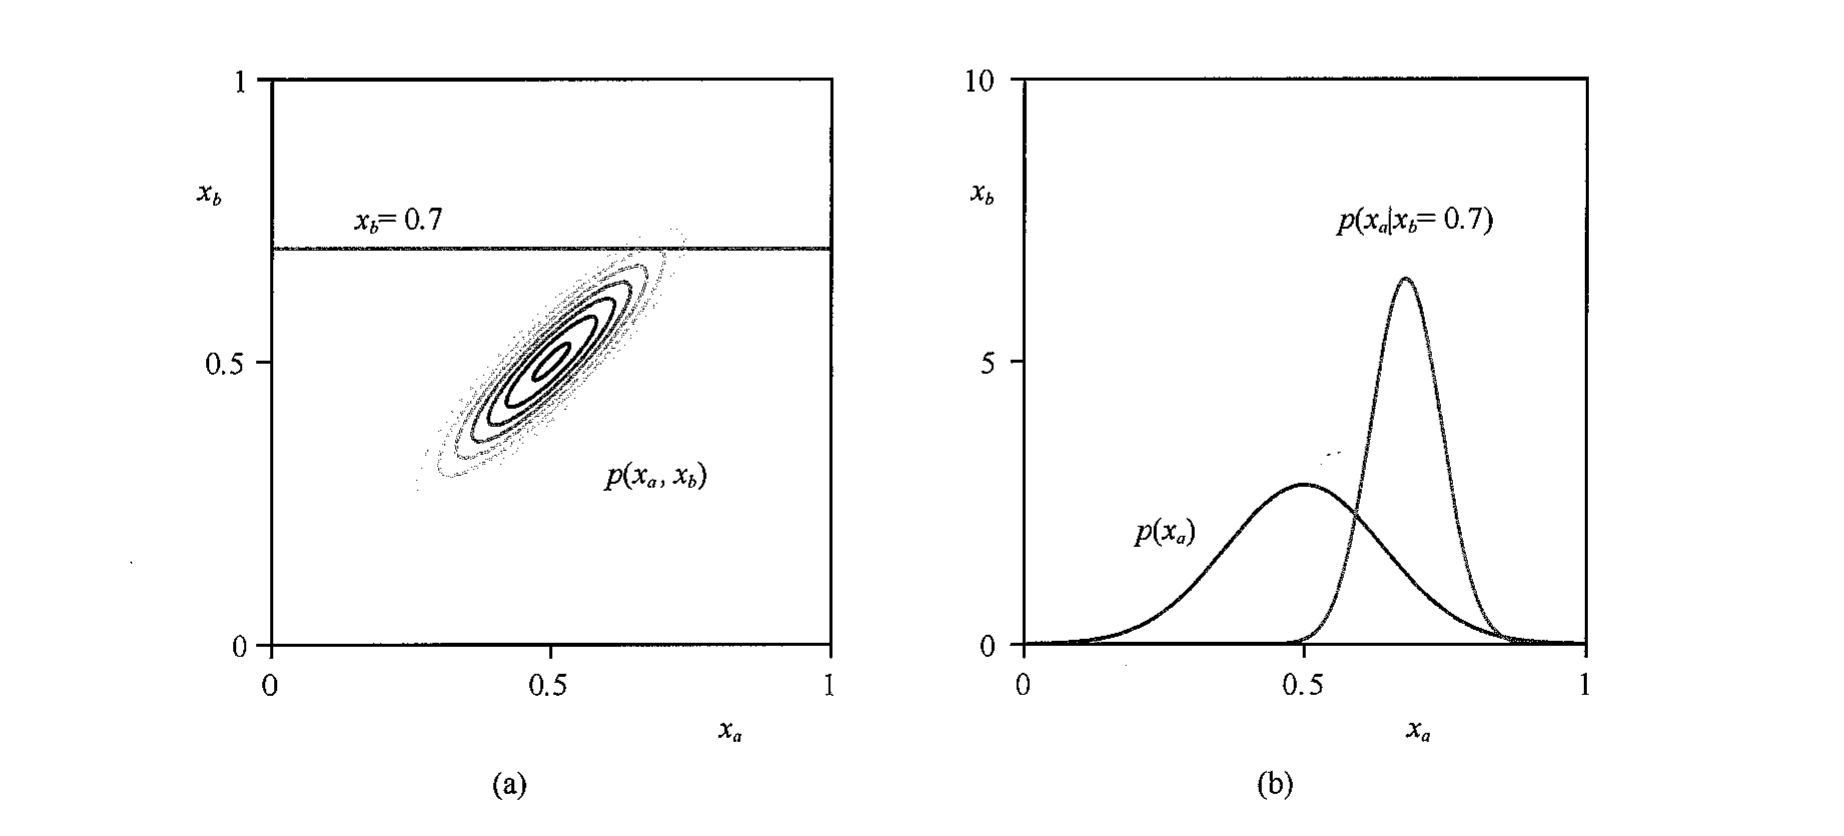
\includegraphics[width=0.92\textwidth]{ch03-fig3-5-marg-cond.png}
  \caption{(a)~一个涉及两个变量的 Gauss 分布 $p(x_a,x_b)$ 的等值线。(b)~$p(x_a)$ 的边缘分布（蓝色曲线）和 $x_b=0.7$ 时的条件分布 $p(x_a\mid x_b)$（红色曲线）。}
  \label{figure:ch03-边缘与条件}
\end{figure}

可以看到，对于边缘分布，均值和协方差用分量协方差矩阵表达最简单；而对于条件分布，均值和协方差用分量精度矩阵表达最简单。

我们可以将分量形式 Gauss 分布的边缘分布和条件分布的结果总结如下。对于联合 Gauss 分布 $\mathcal{N}(\boldsymbol{x}\mid\boldsymbol{\mu},\boldsymbol{\Sigma})$，给定 $\boldsymbol{\Lambda}=\boldsymbol{\Sigma}^{-1}$ 和下列分量矩阵：
\begin{align}
\boldsymbol{x}=\begin{pmatrix}\boldsymbol{x}_{a}\\ \boldsymbol{x}_{b}\end{pmatrix},\qquad
\boldsymbol{\mu}=\begin{pmatrix}\boldsymbol{\mu}_{a}\\ \boldsymbol{\mu}_{b}\end{pmatrix},
\label{align:ch03-分量定义}
\end{align}
\begin{align}
\boldsymbol{\Sigma}=\begin{pmatrix}\boldsymbol{\Sigma}_{aa} & \boldsymbol{\Sigma}_{ab}\\ \boldsymbol{\Sigma}_{ba} & \boldsymbol{\Sigma}_{bb}\end{pmatrix},\qquad
\boldsymbol{\Lambda}=\begin{pmatrix}\boldsymbol{\Lambda}_{aa} & \boldsymbol{\Lambda}_{ab}\\ \boldsymbol{\Lambda}_{ba} & \boldsymbol{\Lambda}_{bb}\end{pmatrix},
\label{align:ch03-分量矩阵}
\end{align}
则条件分布由下式给出：
\begin{align}
p(\boldsymbol{x}_{a}\mid\boldsymbol{x}_{b})=\mathcal{N}\bigl(\boldsymbol{x}\mid\boldsymbol{\mu}_{a\mid b},\boldsymbol{\Lambda}_{aa}^{-1}\bigr),
\label{align:ch03-条件分布总结}
\end{align}
\begin{align}
\boldsymbol{\mu}_{a\mid b}=\boldsymbol{\mu}_{a}-\boldsymbol{\Lambda}_{aa}^{-1}\boldsymbol{\Lambda}_{ab}(\boldsymbol{x}_{b}-\boldsymbol{\mu}_{b}),
\label{align:ch03-条件均值总结}
\end{align}
边缘分布由下式给出：
\begin{align}
p(\boldsymbol{x}_{a})=\mathcal{N}\bigl(\boldsymbol{x}_{a}\mid\boldsymbol{\mu}_{a},\boldsymbol{\Sigma}_{aa}\bigr).
\label{align:ch03-边缘分布总结}
\end{align}
\cref{figure:ch03-边缘与条件}用一个涉及两个变量的示例，对多元 Gauss 分布的边缘分布和条件分布的思想进行了阐释。

\subsection{Bayes定理}\label{subsection:ch03-Bayes定理}

在\cref{subsection:ch03-条件分布}和\cref{subsection:ch03-边缘分布}中，我们考虑了 Gauss 分布 $p(\boldsymbol{x})$，其中我们将向量 $\boldsymbol{x}$ 分成了两个子向量 $\boldsymbol{x}=(\boldsymbol{x}_{a},\boldsymbol{x}_{b})$，然后找到了条件分布 $p(\boldsymbol{x}_{a}\mid\boldsymbol{x}_{b})$ 和边缘分布 $p(\boldsymbol{x}_{a})$ 的表达式。注意条件分布 $p(\boldsymbol{x}_{a}\mid\boldsymbol{x}_{b})$ 的均值是 $\boldsymbol{x}_{b}$ 的线性函数。在这里，假设我们有 Gauss 边缘分布 $p(\boldsymbol{x})$ 和 Gauss 条件分布 $p(\boldsymbol{y}\mid\boldsymbol{x})$，其中 $p(\boldsymbol{y}\mid\boldsymbol{x})$ 的均值是 $\boldsymbol{x}$ 的线性函数，协方差与 $\boldsymbol{x}$ 独立。这是线性-Gauss 模型的一个例子（Roweis and Ghahramani, 1999）（参见\cref{subsection:ch11-Gauss变量}）。我们希望找到边缘分布 $p(\boldsymbol{y})$ 和条件分布 $p(\boldsymbol{x}\mid\boldsymbol{y})$。这种结构在好几种生成式模型中都有出现（参见\cref{chapter:ch16-连续潜变量}），因此在这里推导出一般结论会很有帮助。

我们将边缘分布和条件分布取如下形式：
\begin{align}
p(\boldsymbol{x})=\mathcal{N}(\boldsymbol{x}\mid\boldsymbol{\mu},\boldsymbol{\Lambda}^{-1}),
\label{align:ch03-先验Gauss}
\end{align}
\begin{align}
p(\boldsymbol{y}\mid\boldsymbol{x})=\mathcal{N}(\boldsymbol{y}\mid\boldsymbol{A}\boldsymbol{x}+\boldsymbol{b},\boldsymbol{L}^{-1}),
\label{align:ch03-线性Gauss条件}
\end{align}
其中 $\boldsymbol{\mu}$、$\boldsymbol{A}$ 和 $\boldsymbol{b}$ 是控制均值的参数，$\boldsymbol{\Lambda}$ 和 $\boldsymbol{L}$ 是精度矩阵。如果 $\boldsymbol{x}$ 的维度为 $M$，$\boldsymbol{y}$ 的维度为 $D$，则矩阵 $\boldsymbol{A}$ 的大小为 $D\times M$。

首先找到 $\boldsymbol{x}$ 和 $\boldsymbol{y}$ 上联合分布的表达式。为此，我们定义
\begin{align}
\boldsymbol{z}=\begin{pmatrix}\boldsymbol{x}\\ \boldsymbol{y}\end{pmatrix},
\label{align:ch03-联合变量}
\end{align}
然后考虑联合分布的对数：
\begin{align}
\ln p(\boldsymbol{z})&=\ln p(\boldsymbol{x})+\ln p(\boldsymbol{y}\mid\boldsymbol{x})\nonumber\\
&=-\frac{1}{2}(\boldsymbol{x}-\boldsymbol{\mu})^{\mathsf{T}}\boldsymbol{\Lambda}(\boldsymbol{x}-\boldsymbol{\mu})-\frac{1}{2}(\boldsymbol{y}-\boldsymbol{A}\boldsymbol{x}-\boldsymbol{b})^{\mathsf{T}}\boldsymbol{L}(\boldsymbol{y}-\boldsymbol{A}\boldsymbol{x}-\boldsymbol{b})+\text{const},
\label{align:ch03-联合对数}
\end{align}
其中“const”表示独立于 $\boldsymbol{x}$ 和 $\boldsymbol{y}$ 的常数项。如前所述，这是 $\boldsymbol{z}$ 分量的二次函数，因此 $p(\boldsymbol{z})$ 是 Gauss 分布。为了找到这个 Gauss 分布的精度矩阵，\eqref{align:ch03-联合对数}中的二阶项可以写成
\begin{align}
&-\frac{1}{2}\boldsymbol{x}^{\mathsf{T}}\bigl(\boldsymbol{\Lambda}+\boldsymbol{A}^{\mathsf{T}}\boldsymbol{L}\boldsymbol{A}\bigr)\boldsymbol{x}-\frac{1}{2}\boldsymbol{y}^{\mathsf{T}}\boldsymbol{L}\boldsymbol{y}+\frac{1}{2}\boldsymbol{y}^{\mathsf{T}}\boldsymbol{L}\boldsymbol{A}\boldsymbol{x}+\frac{1}{2}\boldsymbol{x}^{\mathsf{T}}\boldsymbol{A}^{\mathsf{T}}\boldsymbol{L}\boldsymbol{y}\nonumber\\
&\quad=-\frac{1}{2}\begin{pmatrix}\boldsymbol{x}\\ \boldsymbol{y}\end{pmatrix}^{\mathsf{T}}\begin{pmatrix}\boldsymbol{\Lambda}+\boldsymbol{A}^{\mathsf{T}}\boldsymbol{L}\boldsymbol{A} & -\boldsymbol{A}^{\mathsf{T}}\boldsymbol{L}\\ -\boldsymbol{L}\boldsymbol{A} & \boldsymbol{L}\end{pmatrix}\begin{pmatrix}\boldsymbol{x}\\ \boldsymbol{y}\end{pmatrix}=-\frac{1}{2}\boldsymbol{z}^{\mathsf{T}}\boldsymbol{R}\boldsymbol{z},
\label{align:ch03-联合二次型}
\end{align}
因此，$\boldsymbol{z}$ 上的 Gauss 分布的精度（逆协方差）矩阵由下式给出：
\begin{align}
\boldsymbol{R}=\begin{pmatrix}\boldsymbol{\Lambda}+\boldsymbol{A}^{\mathsf{T}}\boldsymbol{L}\boldsymbol{A} & -\boldsymbol{A}^{\mathsf{T}}\boldsymbol{L}\\ -\boldsymbol{L}\boldsymbol{A} & \boldsymbol{L}\end{pmatrix}.
\label{align:ch03-联合精度}
\end{align}
协方差矩阵是通过取精度矩阵的逆矩阵来求的，这可以通过使用逆矩阵公式\eqref{align:ch03-分块逆}来实现（见\cref{exercise:ch03-23}），即
\begin{align}
\mathrm{cov}[\boldsymbol{z}]=\boldsymbol{R}^{-1}=\begin{pmatrix}\boldsymbol{\Lambda}^{-1} & \boldsymbol{\Lambda}^{-1}\boldsymbol{A}^{\mathsf{T}}\\ \boldsymbol{A}\boldsymbol{\Lambda}^{-1} & \boldsymbol{L}^{-1}+\boldsymbol{A}\boldsymbol{\Lambda}^{-1}\boldsymbol{A}^{\mathsf{T}}\end{pmatrix}.
\label{align:ch03-联合协方差}
\end{align}
同样，也可以通过识别\eqref{align:ch03-联合对数}中的线性项来计算关于 $\boldsymbol{z}$ 的 Gauss 分布的均值，它由下式给出：
\begin{align}
\boldsymbol{x}^{\mathsf{T}}\boldsymbol{\Lambda}\boldsymbol{\mu}-\boldsymbol{x}^{\mathsf{T}}\boldsymbol{A}^{\mathsf{T}}\boldsymbol{L}\boldsymbol{b}+\boldsymbol{y}^{\mathsf{T}}\boldsymbol{L}\boldsymbol{b}=\begin{pmatrix}\boldsymbol{x}\\ \boldsymbol{y}\end{pmatrix}^{\mathsf{T}}\begin{pmatrix}\boldsymbol{\Lambda}\boldsymbol{\mu}-\boldsymbol{A}^{\mathsf{T}}\boldsymbol{L}\boldsymbol{b}\\ \boldsymbol{L}\boldsymbol{b}\end{pmatrix}.
\label{align:ch03-联合线性项}
\end{align}
使用我们之前通过在多元 Gauss 分布的二次型上完全平方得到的结果\eqref{align:ch03-完全平方恒等式}，可以发现 $\boldsymbol{z}$ 的均值由下式给出：
\begin{align}
\mathbb{E}[\boldsymbol{z}]=\boldsymbol{R}^{-1}\begin{pmatrix}\boldsymbol{\Lambda}\boldsymbol{\mu}-\boldsymbol{A}^{\mathsf{T}}\boldsymbol{L}\boldsymbol{b}\\ \boldsymbol{L}\boldsymbol{b}\end{pmatrix}.
\label{align:ch03-联合均值}
\end{align}
利用\eqref{align:ch03-联合协方差}（见\cref{exercise:ch03-24}），可以得到
\begin{align}
\mathbb{E}[\boldsymbol{z}]=\begin{pmatrix}\boldsymbol{\mu}\\ \boldsymbol{A}\boldsymbol{\mu}+\boldsymbol{b}\end{pmatrix}.
\label{align:ch03-联合均值化简}
\end{align}

接下来，我们在 $\boldsymbol{x}$ 上进行边缘化，得到 $p(\boldsymbol{y})$ 的表达式。回想一下，当使用分量协方差矩阵来表达服从 Gauss 分布的随机向量子集的边缘分布时，我们可以采用非常简单的形式（参见\cref{subsection:ch03-边缘分布}）。具体来说，其均值和协方差分别由\eqref{align:ch03-边缘均值}和\eqref{align:ch03-边缘协方差}给出。利用\eqref{align:ch03-联合协方差}和\eqref{align:ch03-联合均值化简}可以看到，边缘分布 $p(\boldsymbol{y})$ 的均值和协方差由下式给出：
\begin{align}
\mathbb{E}[\boldsymbol{y}]=\boldsymbol{A}\boldsymbol{\mu}+\boldsymbol{b},
\label{align:ch03-边缘Bayes}
\end{align}
\begin{align}
\mathrm{cov}[\boldsymbol{y}]=\boldsymbol{L}^{-1}+\boldsymbol{A}\boldsymbol{\Lambda}^{-1}\boldsymbol{A}^{\mathsf{T}}.
\label{align:ch03-边缘Bayes协方差}
\end{align}
这个结果的一个特例出现在 $\boldsymbol{A}=\boldsymbol{I}$ 时，在这种情况下，边缘分布退化为两个 Gauss 分布的卷积。由此可以看到，卷积的均值是两个 Gauss 分布的均值之和，卷积的协方差则是它们的协方差之和。

最后推导条件分布 $p(\boldsymbol{x}\mid\boldsymbol{y})$ 的表达式。回想一下，条件分布的结果可以很容易地通过\eqref{align:ch03-条件协方差精度}和\eqref{align:ch03-条件均值精度}，用分量精度矩阵来表示（参见\cref{subsection:ch03-条件分布}）。将这些结果应用于\eqref{align:ch03-联合协方差}和\eqref{align:ch03-联合均值化简}，可以看到条件分布 $p(\boldsymbol{x}\mid\boldsymbol{y})$ 具有以下均值和协方差：
\begin{align}
\mathbb{E}[\boldsymbol{x}\mid\boldsymbol{y}]=\bigl(\boldsymbol{\Lambda}+\boldsymbol{A}^{\mathsf{T}}\boldsymbol{L}\boldsymbol{A}\bigr)^{-1}\bigl\{\boldsymbol{A}^{\mathsf{T}}\boldsymbol{L}(\boldsymbol{y}-\boldsymbol{b})+\boldsymbol{\Lambda}\boldsymbol{\mu}\bigr\},
\label{align:ch03-后验均值}
\end{align}
\begin{align}
\mathrm{cov}[\boldsymbol{x}\mid\boldsymbol{y}]=\bigl(\boldsymbol{\Lambda}+\boldsymbol{A}^{\mathsf{T}}\boldsymbol{L}\boldsymbol{A}\bigr)^{-1}.
\label{align:ch03-后验协方差}
\end{align}

\begin{proposition}[线性-Gauss 模型中的边缘分布与后验分布]\label{proposition:ch03-线性GaussBayes}
设 $p(\boldsymbol{x})=\mathcal{N}(\boldsymbol{x}\mid\boldsymbol{\mu},\boldsymbol{\Lambda}^{-1})$ 与 $p(\boldsymbol{y}\mid\boldsymbol{x})=\mathcal{N}(\boldsymbol{y}\mid\boldsymbol{A}\boldsymbol{x}+\boldsymbol{b},\boldsymbol{L}^{-1})$ 由\eqref{align:ch03-先验Gauss}与\eqref{align:ch03-线性Gauss条件}给出，且 $\boldsymbol{\Lambda},\boldsymbol{L}$ 正定。则边缘分布与条件分布分别为
\begin{align*}
p(\boldsymbol{y})=\mathcal{N}\bigl(\boldsymbol{y}\mid\boldsymbol{A}\boldsymbol{\mu}+\boldsymbol{b},\ \boldsymbol{L}^{-1}+\boldsymbol{A}\boldsymbol{\Lambda}^{-1}\boldsymbol{A}^{\mathsf{T}}\bigr),
\end{align*}
\begin{align*}
p(\boldsymbol{x}\mid\boldsymbol{y})=\mathcal{N}\bigl(\boldsymbol{x}\mid\boldsymbol{\Sigma}\{\boldsymbol{\Lambda}\boldsymbol{\mu}+\boldsymbol{A}^{\mathsf{T}}\boldsymbol{L}(\boldsymbol{y}-\boldsymbol{b})\},\ \boldsymbol{\Sigma}\bigr),
\end{align*}
其中
\begin{align}
\boldsymbol{\Sigma}=\bigl(\boldsymbol{\Lambda}+\boldsymbol{A}^{\mathsf{T}}\boldsymbol{L}\boldsymbol{A}\bigr)^{-1}.
\label{align:ch03-后验协方差形式}
\end{align}
\end{proposition}
\begin{proof}
（重构新增）联合分布的对数由\eqref{align:ch03-联合对数}给出，它是 $\boldsymbol{z}=(\boldsymbol{x},\boldsymbol{y})$ 的二次函数，故联合分布为 Gauss 分布。

由\eqref{align:ch03-联合二次型}读出精度矩阵 $\boldsymbol{R}$（\eqref{align:ch03-联合精度}），再由分块逆公式\eqref{align:ch03-分块逆}求逆。取 $\boldsymbol{A}_{\text{block}}=\boldsymbol{\Lambda}+\boldsymbol{A}^{\mathsf{T}}\boldsymbol{L}\boldsymbol{A}$、$\boldsymbol{B}_{\text{block}}=-\boldsymbol{A}^{\mathsf{T}}\boldsymbol{L}$、$\boldsymbol{C}_{\text{block}}=-\boldsymbol{L}\boldsymbol{A}$、$\boldsymbol{D}_{\text{block}}=\boldsymbol{L}$，则 Schur 补为 $\boldsymbol{M}=(\boldsymbol{\Lambda}+\boldsymbol{A}^{\mathsf{T}}\boldsymbol{L}\boldsymbol{A}-\boldsymbol{A}^{\mathsf{T}}\boldsymbol{L}\boldsymbol{L}^{-1}\boldsymbol{L}\boldsymbol{A})^{-1}=\boldsymbol{\Lambda}^{-1}$，代入\eqref{align:ch03-分块逆}即得\eqref{align:ch03-联合协方差}。

由\eqref{align:ch03-完全平方恒等式}，均值等于协方差矩阵乘以线性项系数。把\eqref{align:ch03-联合协方差}与\eqref{align:ch03-联合线性项}相乘：
\begin{align*}
\boldsymbol{R}^{-1}\begin{pmatrix}\boldsymbol{\Lambda}\boldsymbol{\mu}-\boldsymbol{A}^{\mathsf{T}}\boldsymbol{L}\boldsymbol{b}\\ \boldsymbol{L}\boldsymbol{b}\end{pmatrix}=\begin{pmatrix}\boldsymbol{\Lambda}^{-1}(\boldsymbol{\Lambda}\boldsymbol{\mu}-\boldsymbol{A}^{\mathsf{T}}\boldsymbol{L}\boldsymbol{b})+\boldsymbol{\Lambda}^{-1}\boldsymbol{A}^{\mathsf{T}}\boldsymbol{L}\boldsymbol{b}\\ \boldsymbol{A}\boldsymbol{\Lambda}^{-1}(\boldsymbol{\Lambda}\boldsymbol{\mu}-\boldsymbol{A}^{\mathsf{T}}\boldsymbol{L}\boldsymbol{b})+(\boldsymbol{L}^{-1}+\boldsymbol{A}\boldsymbol{\Lambda}^{-1}\boldsymbol{A}^{\mathsf{T}})\boldsymbol{L}\boldsymbol{b}\end{pmatrix}=\begin{pmatrix}\boldsymbol{\mu}\\ \boldsymbol{A}\boldsymbol{\mu}+\boldsymbol{b}\end{pmatrix},
\end{align*}
即\eqref{align:ch03-联合均值化简}。

于是联合分布为 $\mathcal{N}(\boldsymbol{z}\mid(\boldsymbol{\mu},\boldsymbol{A}\boldsymbol{\mu}+\boldsymbol{b}),\ \mathrm{cov}[\boldsymbol{z}])$。按\cref{proposition:ch03-边缘Gauss}对 $\boldsymbol{x}$ 取边缘，均值为 $\boldsymbol{A}\boldsymbol{\mu}+\boldsymbol{b}$，协方差为 $\boldsymbol{R}^{-1}$ 的右下块 $\boldsymbol{L}^{-1}+\boldsymbol{A}\boldsymbol{\Lambda}^{-1}\boldsymbol{A}^{\mathsf{T}}$，即\eqref{align:ch03-边缘Bayes}与\eqref{align:ch03-边缘Bayes协方差}。

最后按\cref{proposition:ch03-条件Gauss精度}计算 $p(\boldsymbol{x}\mid\boldsymbol{y})$：在分块 $\boldsymbol{z}=(\boldsymbol{x},\boldsymbol{y})$ 下，$\boldsymbol{x}$ 的地位相当于“$\boldsymbol{x}_a$”，$\boldsymbol{y}$ 相当于“$\boldsymbol{x}_b$”。联合精度矩阵为\eqref{align:ch03-联合精度}，故 $\boldsymbol{\Lambda}_{aa}=\boldsymbol{\Lambda}+\boldsymbol{A}^{\mathsf{T}}\boldsymbol{L}\boldsymbol{A}$、$\boldsymbol{\Lambda}_{ab}=-\boldsymbol{A}^{\mathsf{T}}\boldsymbol{L}$、$\boldsymbol{\mu}_{a}=\boldsymbol{\mu}$、$\boldsymbol{\mu}_{b}=\boldsymbol{A}\boldsymbol{\mu}+\boldsymbol{b}$。代入\eqref{align:ch03-条件协方差精度}得 $\mathrm{cov}[\boldsymbol{x}\mid\boldsymbol{y}]=(\boldsymbol{\Lambda}+\boldsymbol{A}^{\mathsf{T}}\boldsymbol{L}\boldsymbol{A})^{-1}$，即\eqref{align:ch03-后验协方差}与\eqref{align:ch03-后验协方差形式}；代入\eqref{align:ch03-条件均值精度}得
\begin{align*}
\mathbb{E}[\boldsymbol{x}\mid\boldsymbol{y}]&=\boldsymbol{\mu}-(\boldsymbol{\Lambda}+\boldsymbol{A}^{\mathsf{T}}\boldsymbol{L}\boldsymbol{A})^{-1}(-\boldsymbol{A}^{\mathsf{T}}\boldsymbol{L})\bigl(\boldsymbol{y}-(\boldsymbol{A}\boldsymbol{\mu}+\boldsymbol{b})\bigr)\\
&=\boldsymbol{\Sigma}\bigl\{\boldsymbol{\Lambda}\boldsymbol{\mu}+\boldsymbol{A}^{\mathsf{T}}\boldsymbol{L}(\boldsymbol{y}-\boldsymbol{b})\bigr\},
\end{align*}
其中 $\boldsymbol{\Sigma}=(\boldsymbol{\Lambda}+\boldsymbol{A}^{\mathsf{T}}\boldsymbol{L}\boldsymbol{A})^{-1}$，这就是\eqref{align:ch03-后验均值}。
\end{proof}

% SUPPLEMENT: parent=proposition:ch03-线性GaussBayes; kind=motivation; location=紧随其后的 remark（重构新增）
\begin{remark}（重构新增）
这组公式是线性-Gauss 模型的“闭合性”定理：Gauss 先验与线性-Gauss 似然的组合在边缘化与条件化下都仍在 Gauss 族内。\eqref{align:ch03-边缘Bayes协方差}中的两项有清晰含义：$\boldsymbol{L}^{-1}$ 是观测噪声的协方差，$\boldsymbol{A}\boldsymbol{\Lambda}^{-1}\boldsymbol{A}^{\mathsf{T}}$ 是先验不确定性经 $\boldsymbol{A}$ 传播后的协方差，二者相加即“不确定性叠加”。

后验协方差\eqref{align:ch03-后验协方差}不依赖于观测值 $\boldsymbol{y}$，这说明观测只改变我们对 $\boldsymbol{x}$ 的“中心位置”，不改变后验的“形状”——这正是线性-Gauss 结构可解析计算的根本原因。后验均值\eqref{align:ch03-后验均值}可以看作先验均值与数据信息的加权折中：$\boldsymbol{\Lambda}\boldsymbol{\mu}$ 把先验“拉回”$\boldsymbol{\mu}$，$\boldsymbol{A}^{\mathsf{T}}\boldsymbol{L}(\boldsymbol{y}-\boldsymbol{b})$ 把估计“拉向”与观测一致的方向。

推导用到 $\boldsymbol{\Lambda}$ 与 $\boldsymbol{L}$ 正定（保证各精度矩阵可逆、Schur 补可逆）。若 $\boldsymbol{A}$ 不是满秩，后验仍然良定义，只是某些方向上的信息完全来自先验。
\end{remark}

这些结果可以总结如下。给定关于 $\boldsymbol{x}$ 的边缘分布和给定 $\boldsymbol{x}$ 时关于 $\boldsymbol{y}$ 的条件分布：
\begin{align}
p(\boldsymbol{x})=\mathcal{N}(\boldsymbol{x}\mid\boldsymbol{\mu},\boldsymbol{\Lambda}^{-1}),
\label{align:ch03-Bayes总结先验}
\end{align}
\begin{align}
p(\boldsymbol{y}\mid\boldsymbol{x})=\mathcal{N}(\boldsymbol{y}\mid\boldsymbol{A}\boldsymbol{x}+\boldsymbol{b},\boldsymbol{L}^{-1}),
\label{align:ch03-Bayes总结条件}
\end{align}
则 $\boldsymbol{y}$ 的边缘分布和给定 $\boldsymbol{y}$ 时 $\boldsymbol{x}$ 的条件分布由下式给出：
\begin{align}
p(\boldsymbol{y})=\mathcal{N}\bigl(\boldsymbol{y}\mid\boldsymbol{A}\boldsymbol{\mu}+\boldsymbol{b},\ \boldsymbol{L}^{-1}+\boldsymbol{A}\boldsymbol{\Lambda}^{-1}\boldsymbol{A}^{\mathsf{T}}\bigr),
\label{align:ch03-Bayes总结边缘}
\end{align}
\begin{align}
p(\boldsymbol{x}\mid\boldsymbol{y})=\mathcal{N}\bigl(\boldsymbol{x}\mid\boldsymbol{\Sigma}\{\boldsymbol{A}^{\mathsf{T}}\boldsymbol{L}(\boldsymbol{y}-\boldsymbol{b})+\boldsymbol{\Lambda}\boldsymbol{\mu}\},\ \boldsymbol{\Sigma}\bigr),
\label{align:ch03-Bayes总结后验}
\end{align}
其中
\begin{align}
\boldsymbol{\Sigma}=\bigl(\boldsymbol{\Lambda}+\boldsymbol{A}^{\mathsf{T}}\boldsymbol{L}\boldsymbol{A}\bigr)^{-1}.
\label{align:ch03-Bayes总结后验协方差}
\end{align}

对这种条件分布进行估计可以看作 Bayes 定理的一个示例。在 Bayes 定理中，我们将 $p(\boldsymbol{x})$ 称为 $\boldsymbol{x}$ 的先验分布。如果观测到变量 $\boldsymbol{y}$，则条件分布 $p(\boldsymbol{x}\mid\boldsymbol{y})$ 表示 $\boldsymbol{x}$ 所对应的后验分布。得到边缘分布和条件分布后，我们可以有效地将联合分布 $p(\boldsymbol{z})=p(\boldsymbol{x})p(\boldsymbol{y}\mid\boldsymbol{x})$ 表示为 $p(\boldsymbol{x}\mid\boldsymbol{y})p(\boldsymbol{y})$ 的形式。

\begin{remark}（重构新增）
这一小节把“先验—似然—后验”的语言落实为具体的 Gauss 公式：\eqref{align:ch03-Bayes总结后验}就是后验分布，\eqref{align:ch03-Bayes总结边缘}是证据（边缘似然），而后验均值与协方差正是\eqref{align:ch03-后验均值}与\eqref{align:ch03-后验协方差}。这一结构在连续潜变量模型中反复出现（\cref{chapter:ch16-连续潜变量}），因为在那里 $\boldsymbol{x}$ 是潜变量、$\boldsymbol{y}$ 是观测，二者正是线性-Gauss 关系。

条件 $\boldsymbol{\Lambda}$、$\boldsymbol{L}$ 正定保证所有协方差可逆；若先验方差趋于无穷（$\boldsymbol{\Lambda}\to0$），后验由数据主导；若观测噪声趋于零（$\boldsymbol{L}\to\infty$），后验退化为对 $\boldsymbol{A}\boldsymbol{x}+\boldsymbol{b}=\boldsymbol{y}$ 的精确求解。
\end{remark}

\subsection{最大似然}\label{subsection:ch03-最大似然}

给定数据集 $X=\{\boldsymbol{x}_1,\cdots,\boldsymbol{x}_N\}$，假设其中的观测值 $\{\boldsymbol{x}_n\}$ 服从多元 Gauss 分布且相互独立，则可以通过最大似然来估计分布的参数。对数似然函数由下式给出：
\begin{align}
\ln p(X\mid\boldsymbol{\mu},\boldsymbol{\Sigma})=-\frac{ND}{2}\ln(2\pi)-\frac{N}{2}\ln\lvert\boldsymbol{\Sigma}\rvert-\frac{1}{2}\sum_{n=1}^{N}(\boldsymbol{x}_n-\boldsymbol{\mu})^{\mathsf{T}}\boldsymbol{\Sigma}^{-1}(\boldsymbol{x}_n-\boldsymbol{\mu}).
\label{align:ch03-Gauss对数似然}
\end{align}
通过简单地重排，可以看到似然函数与数据集相关的部分仅依赖于这两个量：
\begin{align}
\sum_{n=1}^{N}\boldsymbol{x}_n \quad\text{和}\quad \sum_{n=1}^{N}\boldsymbol{x}_n\boldsymbol{x}_n^{\mathsf{T}},
\label{align:ch03-Gauss充分统计量}
\end{align}
这称为 Gauss 分布的充分统计量（sufficient statistic）。使用\cref{section:appA-矩阵导数}中的矩阵求导法则，对数似然关于 $\boldsymbol{\mu}$ 的导数由下式给出：
\begin{align}
\frac{\partial}{\partial\boldsymbol{\mu}}\ln p(X\mid\boldsymbol{\mu},\boldsymbol{\Sigma})=\sum_{n=1}^{N}\boldsymbol{\Sigma}^{-1}(\boldsymbol{x}_n-\boldsymbol{\mu}).
\label{align:ch03-Gauss均值导数}
\end{align}
令导数为零，即可得到均值的最大似然估计解：
\begin{align}
\boldsymbol{\mu}_{\mathrm{ML}}=\frac{1}{N}\sum_{n=1}^{N}\boldsymbol{x}_n,
\label{align:ch03-Gauss均值ML}
\end{align}
这是观测数据点集的平均值。关于 $\boldsymbol{\Sigma}$ 最大化\eqref{align:ch03-Gauss对数似然}可以起到更大的作用。最简单的方法是忽略对称约束，正如所要求的那样，得到的解是对称的（参见\cref{exercise:ch03-28}）。我们在 Magnus and Neudecker（1999）中可以找到对这一结果的替代推导，这些推导显式地施加了对称性和正定性约束。结果正如预期的那样，具有如下形式：
\begin{align}
\boldsymbol{\Sigma}_{\mathrm{ML}}=\frac{1}{N}\sum_{n=1}^{N}(\boldsymbol{x}_n-\boldsymbol{\mu}_{\mathrm{ML}})(\boldsymbol{x}_n-\boldsymbol{\mu}_{\mathrm{ML}})^{\mathsf{T}}.
\label{align:ch03-Gauss协方差ML}
\end{align}
其中涉及 $\boldsymbol{\mu}_{\mathrm{ML}}$，因为这是相对于 $\boldsymbol{\mu}$ 和 $\boldsymbol{\Sigma}$ 联合最大化的结果。注意，$\boldsymbol{\mu}_{\mathrm{ML}}$ 的解[\eqref{align:ch03-Gauss均值ML}]并不依赖于 $\boldsymbol{\Sigma}_{\mathrm{ML}}$，因此我们可以首先估计 $\boldsymbol{\mu}_{\mathrm{ML}}$，然后用它来估计 $\boldsymbol{\Sigma}_{\mathrm{ML}}$。

\begin{proposition}[多元 Gauss 分布的最大似然估计]\label{proposition:ch03-Gauss最大似然}
设 $X=\{\boldsymbol{x}_1,\cdots,\boldsymbol{x}_N\}$ 为来自 $\mathcal{N}(\boldsymbol{x}\mid\boldsymbol{\mu},\boldsymbol{\Sigma})$ 的独立同分布观测，$N\geqslant1$。则对数似然\eqref{align:ch03-Gauss对数似然}关于 $(\boldsymbol{\mu},\boldsymbol{\Sigma})$ 的最大值点由\eqref{align:ch03-Gauss均值ML}与\eqref{align:ch03-Gauss协方差ML}给出，其中 $\boldsymbol{\Sigma}$ 限制在正定矩阵集合上。
\end{proposition}
\begin{proof}
（重构新增）关于 $\boldsymbol{\mu}$：由\eqref{align:ch03-Gauss均值导数}，令其为零得 $\sum_n\boldsymbol{\Sigma}^{-1}(\boldsymbol{x}_n-\boldsymbol{\mu})=0$。由于 $\boldsymbol{\Sigma}^{-1}$ 可逆，两边左乘 $\boldsymbol{\Sigma}$ 得 $\sum_n(\boldsymbol{x}_n-\boldsymbol{\mu})=0$，即 $\boldsymbol{\mu}_{\mathrm{ML}}=\frac{1}{N}\sum_n\boldsymbol{x}_n$，这就是\eqref{align:ch03-Gauss均值ML}。

关于 $\boldsymbol{\Sigma}$：记 $\boldsymbol{S}=\sum_n(\boldsymbol{x}_n-\boldsymbol{\mu}_{\mathrm{ML}})(\boldsymbol{x}_n-\boldsymbol{\mu}_{\mathrm{ML}})^{\mathsf{T}}$。利用 $\sum_n(\boldsymbol{x}_n-\boldsymbol{\mu})(\boldsymbol{x}_n-\boldsymbol{\mu})^{\mathsf{T}}=\boldsymbol{S}+N(\boldsymbol{\mu}_{\mathrm{ML}}-\boldsymbol{\mu})(\boldsymbol{\mu}_{\mathrm{ML}}-\boldsymbol{\mu})^{\mathsf{T}}$（交叉项因 $\sum_n(\boldsymbol{x}_n-\boldsymbol{\mu}_{\mathrm{ML}})=0$ 而消失），并利用迹的循环性 $\boldsymbol{a}^{\mathsf{T}}\boldsymbol{\Sigma}^{-1}\boldsymbol{a}=\mathrm{tr}(\boldsymbol{\Sigma}^{-1}\boldsymbol{a}\boldsymbol{a}^{\mathsf{T}})$，可把\eqref{align:ch03-Gauss对数似然}写成
\begin{align*}
\ln p(X\mid\boldsymbol{\mu}_{\mathrm{ML}},\boldsymbol{\Sigma})=-\frac{ND}{2}\ln(2\pi)-\frac{N}{2}\ln\lvert\boldsymbol{\Sigma}\rvert-\frac{1}{2}\mathrm{tr}\bigl(\boldsymbol{\Sigma}^{-1}\boldsymbol{S}\bigr)-\frac{N}{2}(\boldsymbol{\mu}_{\mathrm{ML}}-\boldsymbol{\mu})^{\mathsf{T}}\boldsymbol{\Sigma}^{-1}(\boldsymbol{\mu}_{\mathrm{ML}}-\boldsymbol{\mu}).
\end{align*}
在 $\boldsymbol{\mu}=\boldsymbol{\mu}_{\mathrm{ML}}$ 处最后一项为零。对 $\boldsymbol{\Sigma}$ 求导（忽略对称约束，把它当作一般矩阵），利用 $\partial\ln\lvert\boldsymbol{\Sigma}\rvert/\partial\boldsymbol{\Sigma}=\boldsymbol{\Sigma}^{-\mathsf{T}}$ 与 $\partial\,\mathrm{tr}(\boldsymbol{\Sigma}^{-1}\boldsymbol{S})/\partial\boldsymbol{\Sigma}=-\boldsymbol{\Sigma}^{-\mathsf{T}}\boldsymbol{S}^{\mathsf{T}}\boldsymbol{\Sigma}^{-\mathsf{T}}$，令导数为零得
\begin{align*}
-\frac{N}{2}\boldsymbol{\Sigma}^{-\mathsf{T}}+\frac{1}{2}\boldsymbol{\Sigma}^{-\mathsf{T}}\boldsymbol{S}^{\mathsf{T}}\boldsymbol{\Sigma}^{-\mathsf{T}}=0\quad\Longrightarrow\quad\boldsymbol{\Sigma}=\frac{1}{N}\boldsymbol{S}^{\mathsf{T}}=\frac{1}{N}\boldsymbol{S},
\end{align*}
最后一步因为 $\boldsymbol{S}$ 对称。这正是\eqref{align:ch03-Gauss协方差ML}。

由于 $\boldsymbol{S}$ 半正定，得到的 $\boldsymbol{\Sigma}_{\mathrm{ML}}$ 半正定；当 $N\geqslant D$ 且数据张满 $\mathbb{R}^{D}$ 时它正定，落在约束集内部。此时 $\ln p$ 关于 $\boldsymbol{\Sigma}$ 在约束集上是凹的（$-\ln\lvert\boldsymbol{\Sigma}\rvert$ 严格凸、$-\mathrm{tr}(\boldsymbol{\Sigma}^{-1}\boldsymbol{S})$ 凸），故该驻点是最大值点。若 $\boldsymbol{S}$ 奇异，则最大值在正定矩阵集合的边界上取到（不存在），此时应把 $\boldsymbol{\Sigma}$ 限制在 $\boldsymbol{S}$ 的值域上，或加入正则化。
\end{proof}

% SUPPLEMENT: parent=proposition:ch03-Gauss最大似然; kind=motivation; location=紧随其后的 remark（重构新增）
\begin{remark}（重构新增）
这两个估计量有明确的统计含义：$\boldsymbol{\mu}_{\mathrm{ML}}$ 就是样本均值（\cref{definition:ch03-样本均值}），$\boldsymbol{\Sigma}_{\mathrm{ML}}$ 就是样本协方差（未作无偏修正）。二者可以分两步计算，因为 $\boldsymbol{\mu}_{\mathrm{ML}}$ 的解不依赖 $\boldsymbol{\Sigma}$，这一“解耦”性质在\cref{exercise:ch03-28}中被进一步利用。

证明中“先忽略对称约束再验证解对称”是一个常用技巧：若把 $\boldsymbol{\Sigma}$ 当作一般矩阵求导，得到的驻点自动对称，因此在对称子空间上也是驻点。但正定性约束不能忽略：$\boldsymbol{S}$ 可能奇异，此时 $\boldsymbol{\Sigma}_{\mathrm{ML}}$ 不可逆，对数似然无定义（$\ln\lvert\boldsymbol{\Sigma}\rvert\to-\infty$），这也是高维（$N<D$）时最大似然失效的原因。此外，$\boldsymbol{S}$ 用的是 $\boldsymbol{\mu}_{\mathrm{ML}}$ 而非真实 $\boldsymbol{\mu}$，这一替换使估计量产生 $-\frac{1}{N}\boldsymbol{\Sigma}$ 量级的偏差（见下一段）。
\end{remark}

如果我们估计真实分布下最大似然解的期望（见\cref{exercise:ch03-29}），则可以得到以下结果：
\begin{align}
\mathbb{E}[\boldsymbol{\mu}_{\mathrm{ML}}]=\boldsymbol{\mu},
\label{align:ch03-均值ML期望}
\end{align}
\begin{align}
\mathbb{E}[\boldsymbol{\Sigma}_{\mathrm{ML}}]=\frac{N-1}{N}\boldsymbol{\Sigma}.
\label{align:ch03-协方差ML期望}
\end{align}
可以看到，均值的最大似然估计期望等于真实均值。但是，协方差的最大似然估计期望小于真实值，因此它是有偏的。通过定义一个不同的估计量 $\tilde{\boldsymbol{\Sigma}}$，可以修正这一偏差，其由下式给出：
\begin{align}
\tilde{\boldsymbol{\Sigma}}=\frac{1}{N-1}\sum_{n=1}^{N}(\boldsymbol{x}_n-\boldsymbol{\mu}_{\mathrm{ML}})(\boldsymbol{x}_n-\boldsymbol{\mu}_{\mathrm{ML}})^{\mathsf{T}}.
\label{align:ch03-无偏协方差}
\end{align}
显然，从\eqref{align:ch03-Gauss协方差ML}和\eqref{align:ch03-协方差ML期望}可以看出，$\tilde{\boldsymbol{\Sigma}}$ 的期望与 $\boldsymbol{\Sigma}$ 的期望相等。

\begin{proposition}[最大似然估计量的期望与无偏修正]\label{proposition:ch03-GaussML期望}
设 $\boldsymbol{x}_1,\cdots,\boldsymbol{x}_N$ 独立同分布于 $\mathcal{N}(\boldsymbol{x}\mid\boldsymbol{\mu},\boldsymbol{\Sigma})$，则\eqref{align:ch03-均值ML期望}与\eqref{align:ch03-协方差ML期望}成立，从而\eqref{align:ch03-无偏协方差}定义的 $\tilde{\boldsymbol{\Sigma}}$ 是 $\boldsymbol{\Sigma}$ 的无偏估计，即 $\mathbb{E}[\tilde{\boldsymbol{\Sigma}}]=\boldsymbol{\Sigma}$。
\end{proposition}
\begin{proof}
（重构新增）第一式：由期望的线性性，$\mathbb{E}[\boldsymbol{\mu}_{\mathrm{ML}}]=\frac{1}{N}\sum_n\mathbb{E}[\boldsymbol{x}_n]=\boldsymbol{\mu}$。

第二式：记 $\boldsymbol{z}_n=\boldsymbol{x}_n-\boldsymbol{\mu}$，则 $\boldsymbol{z}_n$ 相互独立、均值为零、协方差为 $\boldsymbol{\Sigma}$，且 $\boldsymbol{\mu}_{\mathrm{ML}}-\boldsymbol{\mu}=\frac{1}{N}\sum_n\boldsymbol{z}_n$。于是
\begin{align*}
\boldsymbol{S}&\triangleq\sum_{n=1}^{N}(\boldsymbol{x}_n-\boldsymbol{\mu}_{\mathrm{ML}})(\boldsymbol{x}_n-\boldsymbol{\mu}_{\mathrm{ML}})^{\mathsf{T}}=\sum_{n=1}^{N}\Bigl(\boldsymbol{z}_n-\frac{1}{N}\sum_{m}\boldsymbol{z}_m\Bigr)\Bigl(\boldsymbol{z}_n-\frac{1}{N}\sum_{m}\boldsymbol{z}_m\Bigr)^{\mathsf{T}}\\
&=\sum_{n}\boldsymbol{z}_n\boldsymbol{z}_n^{\mathsf{T}}-\frac{1}{N}\Bigl(\sum_{n}\boldsymbol{z}_n\Bigr)\Bigl(\sum_{m}\boldsymbol{z}_m\Bigr)^{\mathsf{T}}.
\end{align*}
取期望，利用 $\mathbb{E}[\boldsymbol{z}_n\boldsymbol{z}_n^{\mathsf{T}}]=\boldsymbol{\Sigma}$ 与独立性（$n\neq m$ 时 $\mathbb{E}[\boldsymbol{z}_n\boldsymbol{z}_m^{\mathsf{T}}]=0$），得
\begin{align*}
\mathbb{E}[\boldsymbol{S}]=N\boldsymbol{\Sigma}-\frac{1}{N}\cdot N\boldsymbol{\Sigma}=(N-1)\boldsymbol{\Sigma}.
\end{align*}
于是 $\mathbb{E}[\boldsymbol{\Sigma}_{\mathrm{ML}}]=\frac{1}{N}\mathbb{E}[\boldsymbol{S}]=\frac{N-1}{N}\boldsymbol{\Sigma}$，即\eqref{align:ch03-协方差ML期望}。

最后由 $\tilde{\boldsymbol{\Sigma}}=\frac{N}{N-1}\boldsymbol{\Sigma}_{\mathrm{ML}}$ 得 $\mathbb{E}[\tilde{\boldsymbol{\Sigma}}]=\frac{N}{N-1}\cdot\frac{N-1}{N}\boldsymbol{\Sigma}=\boldsymbol{\Sigma}$。
\end{proof}

% SUPPLEMENT: parent=proposition:ch03-GaussML期望; kind=motivation; location=紧随其后的 remark（重构新增）
\begin{remark}（重构新增）
偏差的来源是“用 $\boldsymbol{\mu}_{\mathrm{ML}}$ 代替真实 $\boldsymbol{\mu}$”：$\boldsymbol{\mu}_{\mathrm{ML}}$ 本身是数据的函数，会向数据中心“靠近”，从而系统性地压小平方离差，压小的量恰好是 $\frac{1}{N}\boldsymbol{\Sigma}$。除以 $N-1$ 而不是 $N$ 正是为了补偿这一项，这也是统计学中“样本方差分母为 $N-1$”的来源。

条件 $N\geqslant2$ 是 $\tilde{\boldsymbol{\Sigma}}$ 有意义的前提，否则分母为零。注意无偏性只保证期望相等，并不保证 $\tilde{\boldsymbol{\Sigma}}$ 一定正定（当 $N-1<D$ 时它必然奇异），因此在 $N$ 较小、$D$ 较大时仍需正则化。
\end{remark}

\subsection{序贯估计}\label{subsection:ch03-序贯估计}

我们对最大似然解的讨论采用了批处理（batch processing）方法，即一次性考虑整个训练集。也可以使用序贯（sequential）方法，该方法允许一次处理一个数据点，然后将其丢弃。这对于在线应用和大数据非常重要，因为一次性批量处理所有数据在这种情况下是不可行的。

考虑\eqref{align:ch03-Gauss均值ML}给出的最大似然估计的均值 $\boldsymbol{\mu}_{\mathrm{ML}}$，当它建立在 $N$ 个观测值之上时，我们将它表示为 $\boldsymbol{\mu}_{\mathrm{ML}}^{(N)}$。如果我们分解出最末尾的数据点 $\boldsymbol{x}_N$ 的贡献，则可以得到
\begin{align}
\boldsymbol{\mu}_{\mathrm{ML}}^{(N)}&=\frac{1}{N}\sum_{n=1}^{N}\boldsymbol{x}_n\nonumber\\
&=\frac{1}{N}\boldsymbol{x}_N+\frac{1}{N}\sum_{n=1}^{N-1}\boldsymbol{x}_n\nonumber\\
&=\frac{1}{N}\boldsymbol{x}_N+\frac{N-1}{N}\boldsymbol{\mu}_{\mathrm{ML}}^{(N-1)}\nonumber\\
&=\boldsymbol{\mu}_{\mathrm{ML}}^{(N-1)}+\frac{1}{N}\bigl(\boldsymbol{x}_N-\boldsymbol{\mu}_{\mathrm{ML}}^{(N-1)}\bigr).
\label{align:ch03-序贯更新}
\end{align}

\begin{proposition}[样本均值的序贯更新]\label{proposition:ch03-序贯更新}
设 $\boldsymbol{\mu}_{\mathrm{ML}}^{(N)}=\frac{1}{N}\sum_{n=1}^{N}\boldsymbol{x}_n$，则对 $N\geqslant1$ 有递推式\eqref{align:ch03-序贯更新}，即 $\boldsymbol{\mu}_{\mathrm{ML}}^{(N)}=\boldsymbol{\mu}_{\mathrm{ML}}^{(N-1)}+\frac{1}{N}\bigl(\boldsymbol{x}_N-\boldsymbol{\mu}_{\mathrm{ML}}^{(N-1)}\bigr)$。
\end{proposition}
\begin{proof}
（重构新增）由定义，
\begin{align*}
\boldsymbol{\mu}_{\mathrm{ML}}^{(N)}=\frac{1}{N}\Bigl(\sum_{n=1}^{N-1}\boldsymbol{x}_n+\boldsymbol{x}_N\Bigr)=\frac{N-1}{N}\cdot\frac{1}{N-1}\sum_{n=1}^{N-1}\boldsymbol{x}_n+\frac{1}{N}\boldsymbol{x}_N=\frac{N-1}{N}\boldsymbol{\mu}_{\mathrm{ML}}^{(N-1)}+\frac{1}{N}\boldsymbol{x}_N,
\end{align*}
再把它改写为
\begin{align*}
\frac{N-1}{N}\boldsymbol{\mu}_{\mathrm{ML}}^{(N-1)}+\frac{1}{N}\boldsymbol{x}_N=\boldsymbol{\mu}_{\mathrm{ML}}^{(N-1)}+\frac{1}{N}\bigl(\boldsymbol{x}_N-\boldsymbol{\mu}_{\mathrm{ML}}^{(N-1)}\bigr),
\end{align*}
即得\eqref{align:ch03-序贯更新}。初值可取 $\boldsymbol{\mu}_{\mathrm{ML}}^{(0)}=\boldsymbol{0}$（此时 $N=1$ 的递推给出 $\boldsymbol{\mu}_{\mathrm{ML}}^{(1)}=\boldsymbol{x}_1$）。
\end{proof}

% SUPPLEMENT: parent=proposition:ch03-序贯更新; kind=motivation; location=紧随其后的 remark（重构新增）
\begin{remark}（重构新增）
这个结果可以很容易地按如下方式解释。在观测到 $N-1$ 个数据点后，我们用 $\boldsymbol{\mu}_{\mathrm{ML}}^{(N-1)}$ 来估计 $\boldsymbol{\mu}$。而在观测到数据点 $\boldsymbol{x}_N$ 后，我们可以通过将旧的估计值在“误差信号”$(\boldsymbol{x}_N-\boldsymbol{\mu}_{\mathrm{ML}}^{(N-1)})$ 的方向上移动一个较小的量来获得修订后的估计值，这个较小的量与 $1/N$ 成正比。注意，随着 $N$ 的增加，来自后续数据点的贡献会越来越小。

这一递推的实用价值在于它只需保存当前的估计值与已见样本数，而不必保存全部历史数据，因此适用于在线学习与流式数据。它与随机梯度下降的更新形式相似，区别在于步长 $1/N$ 是确定性的、由样本数给出，而不是人为设定的学习率。注意 $N=1$ 时若取初值 $\boldsymbol{0}$，更新式给出的正是 $\boldsymbol{x}_1$，因此递推可以从空集启动。
\end{remark}

\subsection{Gauss 混合}\label{subsection:ch03-Gauss混合}

尽管 Gauss 分布具有一些重要的分析特性，但在用于对真实数据集建模时，它存在很大的局限性。考虑\cref{figure:ch03-老忠实数据}(a) 中的示例，它又称为“Old Faithful”数据集，其中包括美国黄石国家公园老忠实喷泉喷发的 272 个观测值，每个观测值都以分钟为单位给出喷发的持续时间（横轴）和下一次喷发的时间（以分钟为单位）（纵轴）。我们可以看到该数据集形成了两个主要的簇，并且使用简单的 Gauss 分布无法捕捉这种结构。

\begin{figure}[htbp]
  \centering
  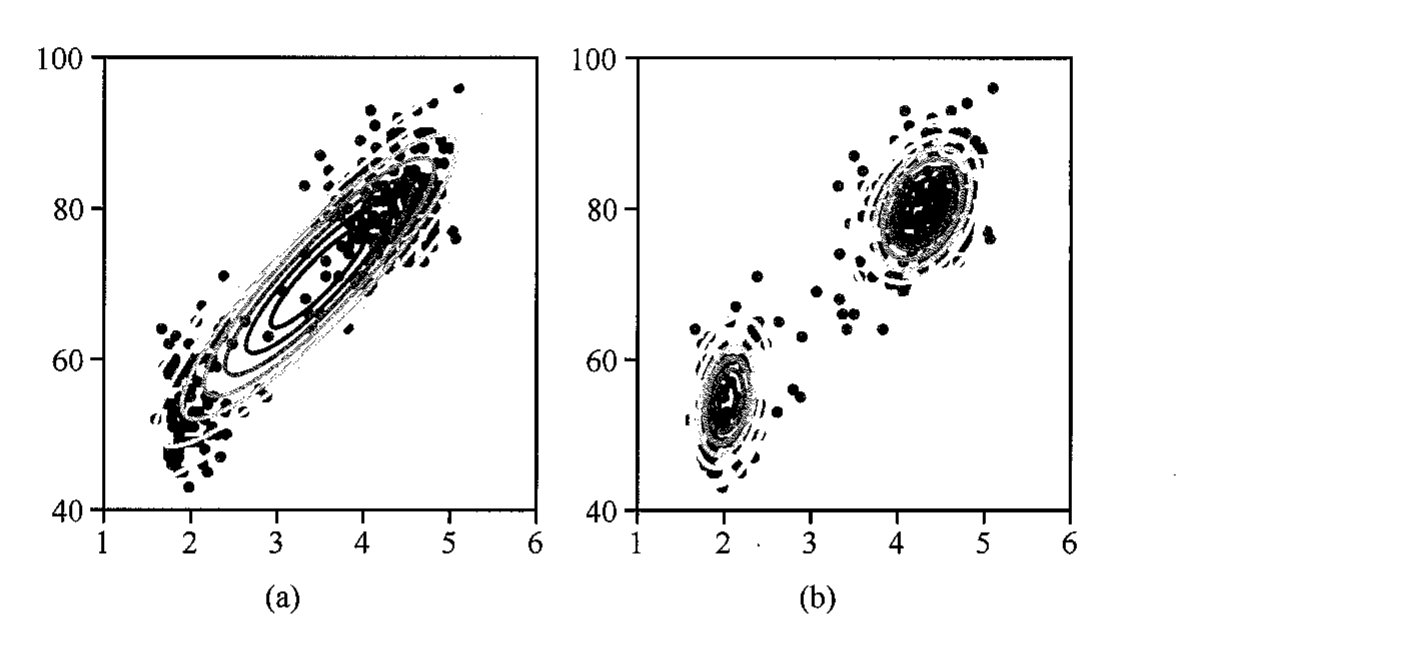
\includegraphics[width=0.82\textwidth]{ch03-fig3-6-old-faithful.png}
  \caption{老忠实喷泉数据的图示，其中红色曲线是等概率密度的等值线。(a)~在单一 Gauss 分布上使用最大似然拟合数据得到的分布。注意，此分布无法捕捉数据中的两个簇，并且确实将其大部分概率质量放置在了数据相对稀疏的团块间的中心区域。(b)~由两个 Gauss 分布的线性组合得到的分布，其也由最大似然拟合，这样可以更好地反映数据。}
  \label{figure:ch03-老忠实数据}
\end{figure}

可以预期，叠加两个 Gauss 分布将能够更好地表示该数据集的结构，情况也确实如此，如\cref{figure:ch03-老忠实数据}(b) 所示。这种叠加是通过对更基本的分布（如 Gauss 分布等）进行线性组合来实现的，可以称作混合分布（mixture distribution）的概率模型（参见\cref{chapter:ch15-离散潜变量}）。在本节中，我们将考虑用 Gauss 分布来说明混合模型的框架。更一般地，混合模型可以包含其他分布的线性组合，例如二元变量的 Bernoulli 分布的混合分布等。在\cref{figure:ch03-一维混合}中，我们看到 Gauss 分布的线性组合可以产生非常复杂的密度。通过使用足够数量的 Gauss 分布，并调整它们的均值、协方差以及线性组合中的系数，我们可以把几乎任何连续分布近似到任意准确度。

\begin{figure}[htbp]
  \centering
  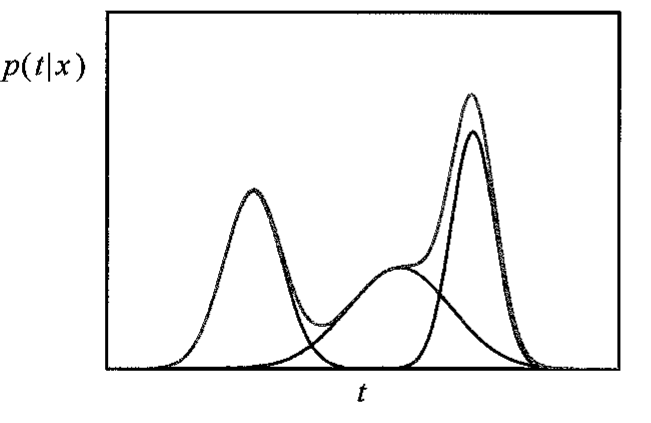
\includegraphics[width=0.52\textwidth]{ch03-fig3-7-mixture-1d.png}
  \caption{一维 Gauss 混合分布，蓝色曲线显示了 3 个 Gauss 分布（每个 Gauss 分布按系数缩放），红色曲线显示了它们的叠加效果。}
  \label{figure:ch03-一维混合}
\end{figure}

考虑形如下式的 $K$ 个 Gauss 密度的叠加：
\begin{align}
p(\boldsymbol{x})=\sum_{k=1}^{K}\pi_{k}\,\mathcal{N}(\boldsymbol{x}\mid\boldsymbol{\mu}_{k},\boldsymbol{\Sigma}_{k}).
\label{align:ch03-Gauss混合}
\end{align}

\begin{definition}[Gauss 混合分布]\label{definition:ch03-Gauss混合}
设 $\pi_1,\cdots,\pi_K$ 满足 $\pi_k\geqslant0$ 与 $\sum_{k=1}^{K}\pi_k=1$，$\mathcal{N}(\boldsymbol{x}\mid\boldsymbol{\mu}_k,\boldsymbol{\Sigma}_k)$ 为第 $k$ 个 Gauss 分量。则称由\eqref{align:ch03-Gauss混合}定义的密度为 Gauss 混合（mixture of Gaussians）。其中每个 Gauss 密度 $\mathcal{N}(\boldsymbol{x}\mid\boldsymbol{\mu}_{k},\boldsymbol{\Sigma}_{k})$ 称为混合的一个分量（component），$\pi_{k}$ 称为混合系数（mixing coefficient）。
\end{definition}

% SUPPLEMENT: parent=definition:ch03-Gauss混合; kind=motivation; location=紧随其后的 remark（重构新增）
\begin{remark}（重构新增）
引入混合分布是为了突破单一 Gauss 分布“单峰”的限制：把若干个 Gauss 密度加权相加，就可以得到多峰的密度，从而描述像 Old Faithful 那样含有多个簇的数据（\cref{figure:ch03-老忠实数据}）。每个分量负责一个簇的位置与形状，混合系数负责各簇的相对权重，因此模型在保持分量形式简单的同时获得了很强的表达能力。

条件 $\pi_k\geqslant0$ 与 $\sum_k\pi_k=1$ 保证 $p(\boldsymbol{x})$ 是合法的概率密度（见\cref{proposition:ch03-混合系数}），各 $\boldsymbol{\Sigma}_k$ 正定保证每个分量良定义。需要注意的是，混合模型的参数个数为 $K-1+K(D+D(D+1)/2)$，随 $K$ 线性增长，因此 $K$ 的选择本身就是一个模型选择问题（\cref{chapter:ch15-离散潜变量}将用最大似然与 EM 算法处理）。
\end{remark}

\cref{figure:ch03-混合等值线}显示了具有 3 个分量的二元 Gauss 混合分布的等值线和曲面图。

\begin{figure}[htbp]
  \centering
  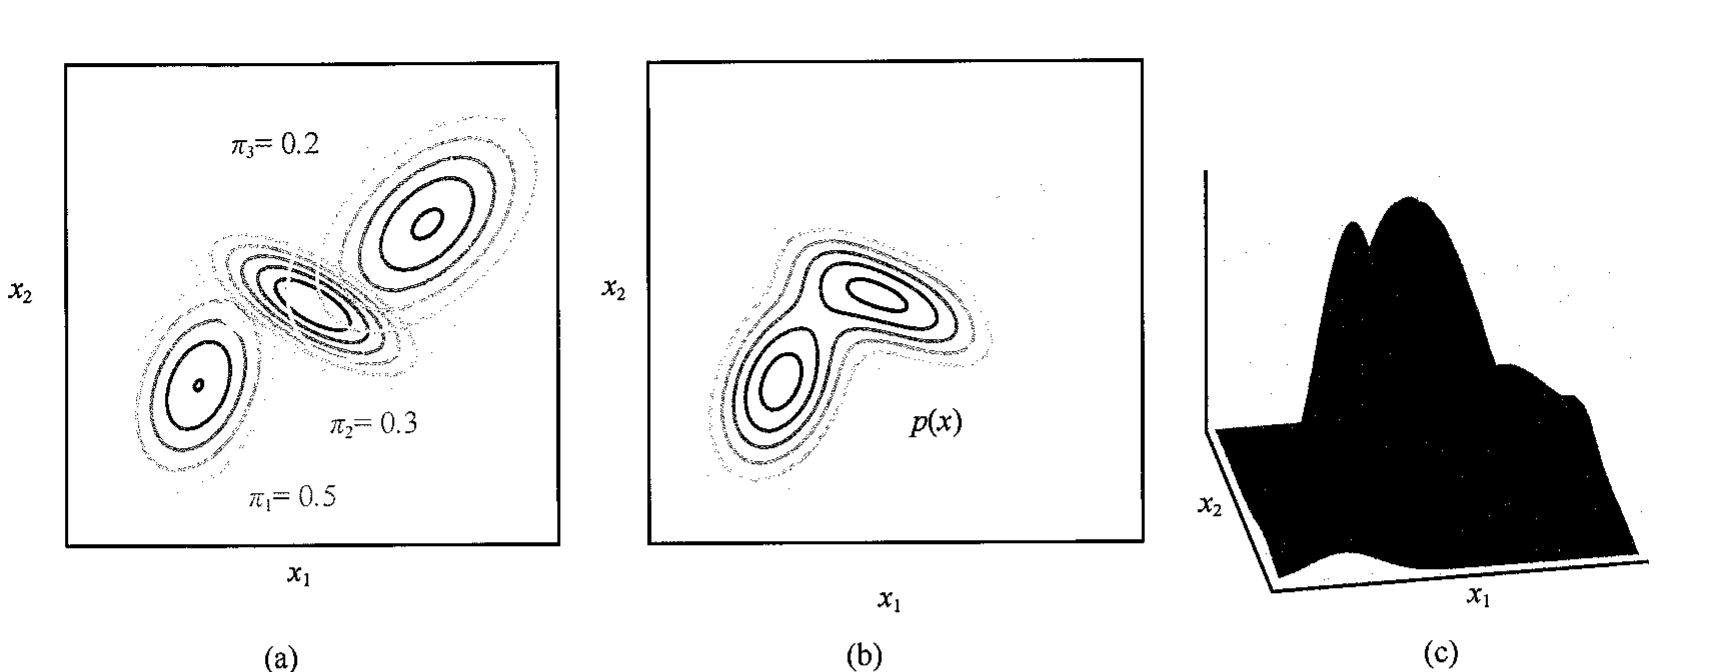
\includegraphics[width=0.95\textwidth]{ch03-fig3-8-mixture-2d.png}
  \caption{3 个二元 Gauss 混合分布的示意图。(a)~每种混合情况的密度等值线，3 种情况分别表示为红色曲线、蓝色曲线和绿色曲线，混合系数的值显示在每个分量的下方。(b)~混合分布的边缘概率密度 $p(\boldsymbol{x})$ 的等值线。(c)~分布 $p(\boldsymbol{x})$ 的曲面图。}
  \label{figure:ch03-混合等值线}
\end{figure}

\eqref{align:ch03-Gauss混合}中的参数 $\pi_{k}$ 称为混合系数（mixing coefficient）。如果在\eqref{align:ch03-Gauss混合}的两边对 $\boldsymbol{x}$ 进行积分，并注意到 $p(\boldsymbol{x})$ 和单个 Gauss 分量都可以归一化，便可得到
\begin{align}
\sum_{k=1}^{K}\pi_{k}=1.
\label{align:ch03-混合系数归一}
\end{align}
此外，给定 $\mathcal{N}(\boldsymbol{x}\mid\boldsymbol{\mu}_{k},\boldsymbol{\Sigma}_{k})\geqslant0$，则 $p(\boldsymbol{x})\geqslant0$ 的充分条件是对所有 $k$ 都有 $\pi_{k}\geqslant0$。将其与条件\eqref{align:ch03-混合系数归一}相结合，可以得到
\begin{align}
0\leqslant\pi_{k}\leqslant1,
\label{align:ch03-混合系数范围}
\end{align}
因此，混合系数满足将其作为概率的要求。

\begin{proposition}[混合系数的归一性与取值范围]\label{proposition:ch03-混合系数}
设 $p(\boldsymbol{x})=\sum_{k=1}^{K}\pi_{k}\mathcal{N}(\boldsymbol{x}\mid\boldsymbol{\mu}_k,\boldsymbol{\Sigma}_k)$ 为 Gauss 混合，各分量归一化。则 $\sum_k\pi_k=1$；若进一步要求 $p(\boldsymbol{x})\geqslant0$ 对一切 $\boldsymbol{x}$ 成立且各 $\pi_k\geqslant0$，则 $0\leqslant\pi_k\leqslant1$。
\end{proposition}
\begin{proof}
（重构新增）对\eqref{align:ch03-Gauss混合}两边关于 $\boldsymbol{x}$ 积分，左边得 $1$（$p$ 是密度），右边由积分的线性性得 $\sum_k\pi_k\int\mathcal{N}(\boldsymbol{x}\mid\boldsymbol{\mu}_k,\boldsymbol{\Sigma}_k)\,\mathrm{d}\boldsymbol{x}=\sum_k\pi_k$，故\eqref{align:ch03-混合系数归一}成立。

若各 $\pi_k\geqslant0$，则 $p(\boldsymbol{x})$ 是若干非负函数之和，必非负；反之若 $p\geqslant0$ 对一切 $\boldsymbol{x}$ 成立，取某个分量的密度远大于其余分量的点即可推出对应 $\pi_k\geqslant0$（严格论证需分量之间线性无关，Gauss 分量一般满足）。结合 $\sum_k\pi_k=1$ 与 $\pi_k\geqslant0$ 得 $0\leqslant\pi_k\leqslant1$，即\eqref{align:ch03-混合系数范围}。
\end{proof}

% SUPPLEMENT: parent=proposition:ch03-混合系数; kind=motivation; location=紧随其后的 remark（重构新增）
\begin{remark}（重构新增）
这两条结论说明混合系数确实可以当作“先验概率”来用：它们非负且和为 $1$，恰好是一个定义在离散变量 $k\in\{1,\cdots,K\}$ 上的概率分布。这正是下一段把 $p(\boldsymbol{x})$ 写成 $\sum_k p(k)p(\boldsymbol{x}\mid k)$ 的依据。

注意“$\pi_k\geqslant0$ 是 $p(\boldsymbol{x})\geqslant0$ 的充分条件”而非必要条件：在一般情况下，让某些 $\pi_k<0$ 而整体仍非负是可能的（只要分量之间相互抵消），但那样混合系数就不再具有概率含义。因此\eqref{align:ch03-混合系数范围}实际上是“把混合系数解释为概率”这一要求的结果，而不是密度非负性的必要条件。
\end{remark}

根据概率的加和法则与乘积法则，边缘密度可以写为
\begin{align}
p(\boldsymbol{x})=\sum_{k=1}^{K}p(k)\,p(\boldsymbol{x}\mid k),
\label{align:ch03-混合生成式}
\end{align}
这等价于\eqref{align:ch03-Gauss混合}，其中可以将 $\pi_{k}=p(k)$ 视为选择第 $k$ 个分量的先验概率，并将密度 $\mathcal{N}(\boldsymbol{x}\mid\boldsymbol{\mu}_{k},\boldsymbol{\Sigma}_{k})=p(\boldsymbol{x}\mid k)$ 视为以 $k$ 为条件时 $\boldsymbol{x}$ 的概率。我们将在后面的章节中看到，相应的后验概率 $p(k\mid\boldsymbol{x})$ 会起到重要作用，因此也称责任。根据 Bayes 定理，这些可以由下式给出：
\begin{align}
\gamma_{k}(\boldsymbol{x})\equiv p(k\mid\boldsymbol{x})=\frac{p(k)\,p(\boldsymbol{x}\mid k)}{\sum_{l}p(l)\,p(\boldsymbol{x}\mid l)}=\frac{\pi_{k}\,\mathcal{N}(\boldsymbol{x}\mid\boldsymbol{\mu}_{k},\boldsymbol{\Sigma}_{k})}{\sum_{l}\pi_{l}\,\mathcal{N}(\boldsymbol{x}\mid\boldsymbol{\mu}_{l},\boldsymbol{\Sigma}_{l})}.
\label{align:ch03-责任}
\end{align}

\begin{definition}[责任]\label{definition:ch03-责任}
在 Gauss 混合\eqref{align:ch03-Gauss混合}中，称由\eqref{align:ch03-责任}定义的后验概率 $\gamma_k(\boldsymbol{x})=p(k\mid\boldsymbol{x})$ 为分量 $k$ 在点 $\boldsymbol{x}$ 处的责任（responsibility）。
\end{definition}

% SUPPLEMENT: parent=definition:ch03-责任; kind=motivation; location=紧随其后的 remark（重构新增）
\begin{remark}（重构新增）
“责任”这一名称来自它的解释：$\gamma_k(\boldsymbol{x})$ 度量的是“观测到 $\boldsymbol{x}$ 之后，把这一点归因于第 $k$ 个分量的可信程度”。它满足 $\gamma_k(\boldsymbol{x})\in[0,1]$ 与 $\sum_k\gamma_k(\boldsymbol{x})=1$，因此可以看作对数据点的一种“软分配”（soft assignment），与 $K$ 均值算法中的硬分配相对应（\cref{chapter:ch15-离散潜变量}）。

责任的定义只用到 Bayes 定理与全概率公式，因此对任意混合分布都成立，并不限于 Gauss 分量。条件 $\sum_l\pi_l\mathcal{N}(\boldsymbol{x}\mid\boldsymbol{\mu}_l,\boldsymbol{\Sigma}_l)>0$ 是分母非零的保证；由于各分量密度严格为正，只要某个 $\pi_l>0$ 该条件就满足。
\end{remark}

通过使用足够数量的 Gauss 分布，并调整它们的均值、协方差以及线性组合中的系数，我们可以把几乎任何连续分布近似到任意准确度。下面我们将证明这种对混合分布的概率解释是非常强大的（参见\cref{chapter:ch15-离散潜变量}）。

\begin{proposition}[混合密度的对数似然]\label{proposition:ch03-混合对数似然}
设 $X=\{\boldsymbol{x}_1,\cdots,\boldsymbol{x}_N\}$ 为独立观测，混合参数为 $\boldsymbol{\pi}=\{\pi_1,\cdots,\pi_K\}$、$\boldsymbol{\mu}=\{\boldsymbol{\mu}_1,\cdots,\boldsymbol{\mu}_K\}$、$\boldsymbol{\Sigma}=\{\boldsymbol{\Sigma}_1,\cdots,\boldsymbol{\Sigma}_K\}$，则对数似然为
\begin{align}
\ln p(X\mid\boldsymbol{\pi},\boldsymbol{\mu},\boldsymbol{\Sigma})=\sum_{n=1}^{N}\ln\left\{\sum_{k=1}^{K}\pi_{k}\,\mathcal{N}(\boldsymbol{x}_n\mid\boldsymbol{\mu}_{k},\boldsymbol{\Sigma}_{k})\right\}.
\label{align:ch03-混合对数似然}
\end{align}
\end{proposition}
\begin{proof}
（重构新增）由独立性与\eqref{align:ch03-Gauss混合}，
\begin{align*}
p(X\mid\boldsymbol{\pi},\boldsymbol{\mu},\boldsymbol{\Sigma})=\prod_{n=1}^{N}p(\boldsymbol{x}_n)=\prod_{n=1}^{N}\sum_{k=1}^{K}\pi_{k}\mathcal{N}(\boldsymbol{x}_n\mid\boldsymbol{\mu}_k,\boldsymbol{\Sigma}_k),
\end{align*}
两边取对数即得\eqref{align:ch03-混合对数似然}。
\end{proof}

% SUPPLEMENT: parent=proposition:ch03-混合对数似然; kind=motivation; location=紧随其后的 remark（重构新增）
\begin{remark}（重构新增）
与单个 Gauss 分布的情形相比，\eqref{align:ch03-混合对数似然}的困难在于对数之内还有对 $k$ 的求和，因此对数不能逐项拆开，参数的最大似然解不再具有闭式表达。这正是混合模型必须借助迭代数值优化（尤其是期望最大化算法）的原因，也是\cref{chapter:ch15-离散潜变量}引入潜变量视角的动机：把“每个点属于哪个分量”视为缺失数据后，完全数据的对数似然就能重新分解为逐分量之和。

条件“各观测独立”只用于把联合密度写成乘积；混合结构本身（求和号在乘积之内）才是非线性的来源。若 $K=1$，\eqref{align:ch03-混合对数似然}退化为单个 Gauss 分布的对数似然\eqref{align:ch03-Gauss对数似然}。
\end{remark}

\end{document}
